% ============================================================
%  FEDCARDIO PROJECT REPORT
%  Using amritareport.cls
%  Keep amritareport.cls in the same folder as this file.
% ============================================================

\documentclass[12pt,a4paper]{amritareport}

% ---------- Additional Essential Packages ----------
\usepackage{amsmath,amssymb,amsfonts}
\usepackage{graphicx}
\graphicspath{{report_images/}{./}}
\usepackage{booktabs}
\usepackage{multirow}
\usepackage{longtable}
\usepackage{array}
\usepackage{algorithm}
\usepackage{algorithmic}
\usepackage{url}
\usepackage[hidelinks]{hyperref}

\reporttitle{FEDCARDIO: CROSS-MODAL FEDERATED PROTOTYPE LEARNING FOR PRIVACY-PRESERVING PEDIATRIC CARDIAC SCREENING}

\degreename{BACHELOR OF TECHNOLOGY IN COMPUTER AND COMMUNICATION ENGINEERING}

\reportdate{October 2026}

\deptaddress{Department of ECE, \\ Amrita School of Engineering,\\ Amrita Vishwa Vidyapeetham, Chennai.}


% ============================================================
% CANDIDATES
% ============================================================

\addcandidate{A ALLAN}{CH.EN.U4CCE23001}
\addcandidate{SURIYA K S}{CH.EN.U4CCE23050}


% ============================================================
% SUPERVISOR AND HOD
% ============================================================

\supervisor{Dr. N. AISHWARYA}{Mentor}
\hod{Dr. LAKSHMANAN S A}{Associate Professor}


% ============================================================
% UNIVERSITY LOGOS
% ============================================================

\universitylogo{Amrita_Logo.png}
\universityfulllogo{Amrita_Full_Logo.png}


% ============================================================
% CORRECTED COVER PAGE SPACING
% ============================================================

\makeatletter

\renewcommand{\makecoverpage}{%
\begin{titlepage}
\begin{center}
\onehalfspacing

{\fontsize{18}{22}\selectfont\bfseries \@reporttitle \par}

\vspace{0.55cm}

{\large\bfseries A PROJECT REPORT\par}

\vspace{0.55cm}

{\large\itshape Submitted by\par}

\vspace{0.10cm}

\@candidatelist

\vspace{0.45cm}

{\large\itshape\bfseries
in partial fulfillment for the award of the degree of\par}

\vspace{0.45cm}

{\large\bfseries \@degreename \par}

\vspace{0.60cm}

{\large\itshape Under the guidance of\par}

\vspace{0.15cm}

{\large\bfseries \@supervisorname \par}

\vspace{0.60cm}

{\large\itshape Submitted to\par}

\vspace{0.15cm}

\ifdefempty{\@universitylogo}
{}
{\includegraphics[width=6cm]{\@universitylogo}\\[0.10cm]}

{\large\bfseries AMRITA SCHOOL OF ENGINEERING\par}

{\large\bfseries AMRITA VISHWA VIDYAPEETHAM\par}

{\large\bfseries CHENNAI -- 601103\par}

\vspace{0.20cm}

{\large\bfseries \@reportdate \par}

\end{center}
\end{titlepage}
}

\makeatother


% ============================================================
% DOCUMENT
% ============================================================

\begin{document}


% ============================================================
% COVER PAGE
% ============================================================

\makecoverpage


% ============================================================
% FRONT MATTER
% ============================================================

\pagenumbering{roman}

\makebonafidecertificate

\makedeclaration


% ============================================================
% ABSTRACT
% ============================================================

\reportabstract{
	Congenital heart disease (CHD) represents one of the leading global causes of infant mortality, affecting approximately 8 to 12 infants per 1,000 live births. Timely, accurate clinical screening in early childhood is vital to avert irreversible physiological deterioration and enable curative surgical interventions. Modern pediatric cardiology utilizes three primary non-invasive diagnostic modalities: phonocardiography (PCG), which records acoustic heart sounds and murmurs; electrocardiography (ECG), which captures electrical cardiac conduction and rhythm; and echocardiography (Echo), which provides spatial-temporal visualization of myocardial wall motion, chamber anatomy, and ejection fraction (EF). 

	In real-world healthcare ecosystems, severe structural inequalities dictate diagnostic equipment availability across clinical institutions. Resource-constrained rural clinics often possess only digital stethoscopes (PCG); secondary district hospitals routinely deploy multi-lead electrocardiographs (ECG); and advanced tertiary referral centers maintain high-end transthoracic echocardiography imaging suites (Echo). Crucially, stringent privacy regulations, including the Health Insurance Portability and Accountability Act (HIPAA), the General Data Protection Regulation (GDPR), and institutional ethics protocols, strictly prohibit the centralized pooling and inter-hospital exchange of confidential pediatric patient records. Furthermore, single-center models trained on isolated local cohorts suffer from constrained demographic diversity and high false-negative screening risks.

	Although federated learning (FL) offers a mathematical paradigm for collaborative model optimization without raw data sharing, conventional federated architectures (e.g., FedAvg, FedProx) rely fundamentally upon homogeneous neural network parameters. Consequently, they completely collapse in cross-modal healthcare environments where participating hospitals maintain structurally incompatible neural architectures (2D audio CNNs, 1D residual temporal networks, and 2D vision backbones) processing entirely disjoint signal spaces.

	To resolve this fundamental dilemma, this dissertation presents \textbf{FedCardio}, an innovative Cross-Modal Federated Prototype Learning framework (CrossFedProto) designed specifically for privacy-preserving pediatric cardiac screening. Under FedCardio, each healthcare institution trains a modality-specific feature encoder locally and projects its latent representations into a compact, shared geometric alignment space ($\mathbb{R}^{64}$) via a lightweight, learnable projection head. Rather than exchanging massive model weight tensors or raw clinical data, clients communicate solely class-level prototype centroids (merely 128 floating-point values per round) to a central aggregation server. The central server computes square-root sample-weighted global prototype anchors and redistributes them to client institutions. Local training is governed by a novel dual prototype objective that integrates class-weighted directional prototype alignment on the unit hypersphere with InfoNCE-based contrastive prototype separation, completely preventing prototype collapse across disparate modalities.

	The proposed framework is rigorously evaluated on three public, multi-center pediatric cardiac cohorts comprising a total of 28,610 clinical samples: CirCor DigiScope (PCG, $n=11,162$ segments), ZZU-pECG (ECG, $n=14,190$ recordings), and EchoNet-Pediatric (Echo, $n=3,258$ frame pairs). Comprehensive empirical benchmarking demonstrates that CrossFedProto matches or exceeds isolated single-center models across all screening metrics while driving inter-modality prototype cosine distances from 1.06 down to less than 0.001 within eight federated rounds. Specifically, the ECG client achieves a statistically significant AUROC surge from 0.9461 to 0.9594 (+1.33\%) alongside a +6.87\% boost in clinical specificity; the PCG client achieves a critical sensitivity surge from 82.62\% to 89.46\% (+6.84\%), drastically reducing missed defects in rural triage; and the Echo client successfully overcomes severe 85:15 class imbalance. Furthermore, FedCardio achieves an astounding 87,800-fold reduction in communication bandwidth compared to conventional FedAvg, requiring only 512 bytes per round. An Explainable AI (XAI) engine utilizing Grad-CAM is integrated to provide clinicians with precise temporal murmur localization. Finally, an enterprise-grade full-stack clinical platform, comprising a high-performance FastAPI asynchronous backend and an interactive React/Vite visualization dashboard, is engineered to demonstrate seamless real-world clinical deployment.

	\noindent\textbf{Keywords:} Congenital Heart Disease, Cross-Modal Federated Learning, Prototype Representation Learning, Pediatric Cardiac Screening, Phonocardiography, Electrocardiography, Echocardiography, Explainable AI, Privacy Preservation
}


% ============================================================
% ACKNOWLEDGEMENT
% ============================================================

\acknowledgement{
	The completion of this Bachelor of Technology project report represents a major academic and intellectual milestone, which has been achieved through the invaluable guidance, unwavering support, and encouragement of several esteemed individuals and institutions.

	First and foremost, we express our deepest sense of gratitude and sincere respect to our project supervisor and mentor, \textbf{Dr. N. Aishwarya}, Assistant Professor, Department of Electronics and Communication Engineering, Amrita School of Engineering, Chennai. Her insightful guidance, patient critique, continuous encouragement, and profound technical acumen throughout the conceptualization, mathematical formulation, and experimental phases have been the foundational pillars of this research work.

	We extend our heartfelt gratitude to \textbf{Dr. Lakshmanan S A}, Associate Professor and Head of the Department, Department of Electronics and Communication Engineering, Amrita School of Engineering, Chennai, for providing us with the state-of-the-art computational infrastructure, institutional resources, and an academically stimulating environment that fostered the successful execution of this multidisciplinary investigation.

	We are immensely thankful to the faculty members, laboratory instructors, and administrative staff of the Department of Electronics and Communication Engineering, Amrita Vishwa Vidyapeetham, Chennai, for their timely administrative assistance, scholastic input, and continuous goodwill.

	We acknowledge with sincere gratitude the creators and open-access research curators of the public biomedical datasets utilized in this investigation: the CirCor DigiScope team, the First Affiliated Hospital of Zhengzhou University (ZZU-pECG team), and Stanford Medicine's AIMI Center (EchoNet-Pediatric team). Their noble commitment to open science and pediatric healthcare data accessibility made this cross-institutional study feasible.

	Finally, we express our profound gratitude to our beloved parents, family members, and peers for their unconditional love, moral support, and endless sacrifices throughout our undergraduate journey. Their unshakeable belief in our potential has been our constant source of inspiration and strength.

	\vspace{1.5cm}
	\begin{flushright}
		\textbf{A ALLAN} \\
		\textbf{SURIYA K S}
	\end{flushright}
}


% ============================================================
% TABLE OF CONTENTS
% LIST OF TABLES
% LIST OF FIGURES
% ============================================================

\frontmattertoc


% ============================================================
% ABBREVIATIONS
% ============================================================

\begin{abbreviations}

\textbf{AI} & - \quad & Artificial Intelligence \\

\textbf{AP4C} & - \quad & Apical Four-Chamber View \\

\textbf{ASD} & - \quad & Atrial Septal Defect \\

\textbf{ASE} & - \quad & American Society of Echocardiography \\

\textbf{AUROC} & - \quad & Area Under the Receiver Operating Characteristic Curve \\

\textbf{AUPRC} & - \quad & Area Under the Precision-Recall Curve \\

\textbf{Bi-LSTM} & - \quad & Bidirectional Long Short-Term Memory Network \\

\textbf{CE} & - \quad & Cross-Entropy Loss \\

\textbf{CHD} & - \quad & Congenital Heart Disease \\

\textbf{CLIP} & - \quad & Contrastive Language-Image Pretraining \\

\textbf{CoA} & - \quad & Coarctation of the Aorta \\

\textbf{CNN} & - \quad & Convolutional Neural Network \\

\textbf{CVD} & - \quad & Cardiovascular Disease \\

\textbf{CWT} & - \quad & Continuous Wavelet Transform \\

\textbf{DL} & - \quad & Deep Learning \\

\textbf{DP} & - \quad & Differential Privacy \\

\textbf{DPDPA} & - \quad & Digital Personal Data Protection Act \\

\textbf{ECG} & - \quad & Electrocardiography / Electrocardiogram \\

\textbf{Echo} & - \quad & Echocardiography / Echocardiogram \\

\textbf{ED} & - \quad & End-Diastole / End-Diastolic Frame \\

\textbf{EF} & - \quad & Ejection Fraction \\

\textbf{ES} & - \quad & End-Systole / End-Systolic Frame \\

\textbf{FDA} & - \quad & Food and Drug Administration \\

\textbf{FedAvg} & - \quad & Federated Averaging Algorithm \\

\textbf{FedCardio} & - \quad & Cross-Modal Federated Pediatric Cardiac Screening Framework \\

\textbf{FedProto} & - \quad & Federated Prototype Learning \\

\textbf{FedProx} & - \quad & Federated Proximal Algorithm \\

\textbf{FL} & - \quad & Federated Learning \\

\textbf{FPR} & - \quad & False Positive Rate \\

\textbf{GAP} & - \quad & Global Average Pooling \\

\textbf{GDPR} & - \quad & General Data Protection Regulation \\

\textbf{Grad-CAM} & - \quad & Gradient-Weighted Class Activation Mapping \\

\textbf{HIPAA} & - \quad & Health Insurance Portability and Accountability Act \\

\textbf{ICD-10} & - \quad & International Classification of Diseases, 10th Revision \\

\textbf{InfoNCE} & - \quad & Information Noise-Contrastive Estimation \\

\textbf{IRB} & - \quad & Institutional Review Board \\

\textbf{L1 / L2} & - \quad & First / Second Norm Distance \\

\textbf{LV} & - \quad & Left Ventricle / Left Ventricular \\

\textbf{LVEF} & - \quad & Left Ventricular Ejection Fraction \\

\textbf{MCC} & - \quad & Matthews Correlation Coefficient \\

\textbf{MFCC} & - \quad & Mel-Frequency Cepstral Coefficients \\

\textbf{ML} & - \quad & Machine Learning \\

\textbf{MLP} & - \quad & Multi-Layer Perceptron \\

\textbf{NPV} & - \quad & Negative Predictive Value \\

\textbf{PCG} & - \quad & Phonocardiography / Phonocardiogram \\

\textbf{PDA} & - \quad & Patent Ductus Arteriosus \\

\textbf{PPV} & - \quad & Positive Predictive Value \\

\textbf{PR} & - \quad & Precision-Recall \\

\textbf{ReLU} & - \quad & Rectified Linear Unit \\

\textbf{ResNet} & - \quad & Residual Neural Network \\

\textbf{ROC} & - \quad & Receiver Operating Characteristic \\

\textbf{S1 / S2} & - \quad & First / Second Heart Sound \\

\textbf{SCAFFOLD} & - \quad & Stochastic Controlled Averaging for Federated Learning \\

\textbf{STFT} & - \quad & Short-Time Fourier Transform \\

\textbf{ToF} & - \quad & Tetralogy of Fallot \\

\textbf{TPR} & - \quad & True Positive Rate \\

\textbf{t-SNE} & - \quad & t-Distributed Stochastic Neighbor Embedding \\

\textbf{VSD} & - \quad & Ventricular Septal Defect \\

\textbf{WFDB} & - \quad & Waveform Database Software Package \\

\textbf{XAI} & - \quad & Explainable Artificial Intelligence \\

\end{abbreviations}


% ============================================================
% START MAIN MATTER
% ============================================================

\startmainmatter


% ============================================================
% CHAPTER 1 - INTRODUCTION
% ============================================================

\chapter{INTRODUCTION}

\section{PEDIATRIC CARDIAC HEALTH AND CONGENITAL HEART DEFECTS}

Congenital heart disease (CHD) represents the most common class of major congenital anomalies encountered in clinical pediatrics, comprising approximately one-third of all major congenital birth defects diagnosed globally. Epidemiological investigations establish that CHD affects between 8 and 12 infants per 1,000 live births worldwide, accounting for over 1.35 million newborns diagnosed with structural cardiac malformations each year \cite{liu2019global, hoffman2002incidence}. In low- and middle-income countries, as well as medically underserved rural territories within developed economies, CHD remains a devastating primary contributor to neonatal, infant, and early childhood morbidity and mortality \cite{zimmerman2020global}. 

The spectrum of structural defects encompassed by CHD spans a wide range of anatomical and hemodynamic abnormalities. These anomalies are broadly categorized into acyanotic and cyanotic lesions:
\begin{enumerate}
	\item \textbf{Ventricular Septal Defect (VSD):} An abnormal opening in the interventricular septum permitting oxygenated blood to shunt from the high-pressure left ventricle into the low-pressure right ventricle. VSD constitutes approximately 30\% to 35\% of all diagnosed congenital cardiac anomalies. Chronic left-to-right shunting causes progressive pulmonary arterial hypertension, right ventricular volume overload, and eventual irreversible congestive heart failure if uncorrected \cite{minette2006ventricular}.
	\item \textbf{Atrial Septal Defect (ASD):} A persistent communication within the interatrial septum, most frequently within the ostium secundum region. ASD allows systemic arterial blood to recirculate through the right atrium and pulmonary vasculature, precipitating right atrial dilation, supraventricular arrhythmias, and secondary tricuspid regurgitation over developmental childhood \cite{webb2006atrial}.
	\item \textbf{Patent Ductus Arteriosus (PDA):} Failure of the physiological fetal vascular bridge between the proximal descending aorta and the main pulmonary artery to close spontaneously following parturition. Persistent PDA generates a continuous acoustic machinery murmur, precipitating significant left heart volume loading and pulmonary hyperperfusion, particularly in premature neonates \cite{benitz2016patent}.
	\item \textbf{Coarctation of the Aorta (CoA):} A discrete pathological narrowing of the aortic lumen typically situated adjacent to the insertion of the ductus arteriosus. CoA creates a severe mechanical pressure gradient between the upper and lower extremities, manifesting as systemic upper-body arterial hypertension, diminished or absent femoral arterial pulses, compensatory left ventricular hypertrophy, and heightened risk of early aortic dissection or stroke \cite{ward2000coarctation}.
	\item \textbf{Tetralogy of Fallot (ToF):} The most prevalent cyanotic congenital anomaly, characterized by four hallmark anatomical hallmarks: a large subaortic ventricular septal defect, severe pulmonary infundibular stenosis, an overriding aorta, and secondary right ventricular concentric hypertrophy. Right-to-left shunting delivers deoxygenated blood directly into systemic circulation, manifesting clinically as episodic hypoxic spells (tet spells), marked cyanosis, and polycythemia \cite{bailliard2009tetralogy}.
\end{enumerate}

Despite the life-threatening severity of these conditions, contemporary advances in pediatric cardiovascular surgery, interventional catheterization, and pharmacological management have rendered more than 85\% of CHD anomalies treatable or curable, enabling affected children to attain normal adult life expectancies \cite{bouma2017changing}. However, this clinical success hinges upon a decisive clinical prerequisite: \textit{early, timely, and systematic cardiac screening}. In the absence of early screening, infants suffering from critical, ductal-dependent, or severe shunt lesions frequently experience acute circulatory collapse, irreversible pulmonary vascular remodeling, severe neurodevelopmental impairment, or premature death prior to formal cardiology consultation.


\section{CLINICAL SCREENING MODALITIES AND DIAGNOSTIC TRIAGE}

The early detection of congenital heart defects relies upon non-invasive physiological diagnostic modalities. In contemporary pediatric practice, three complementary diagnostic tools form the bedrock of cardiac screening: Phonocardiography, Electrocardiography, and Echocardiography \cite{garcia2013comparison}.

\begin{figure}[htbp]
	\centering
	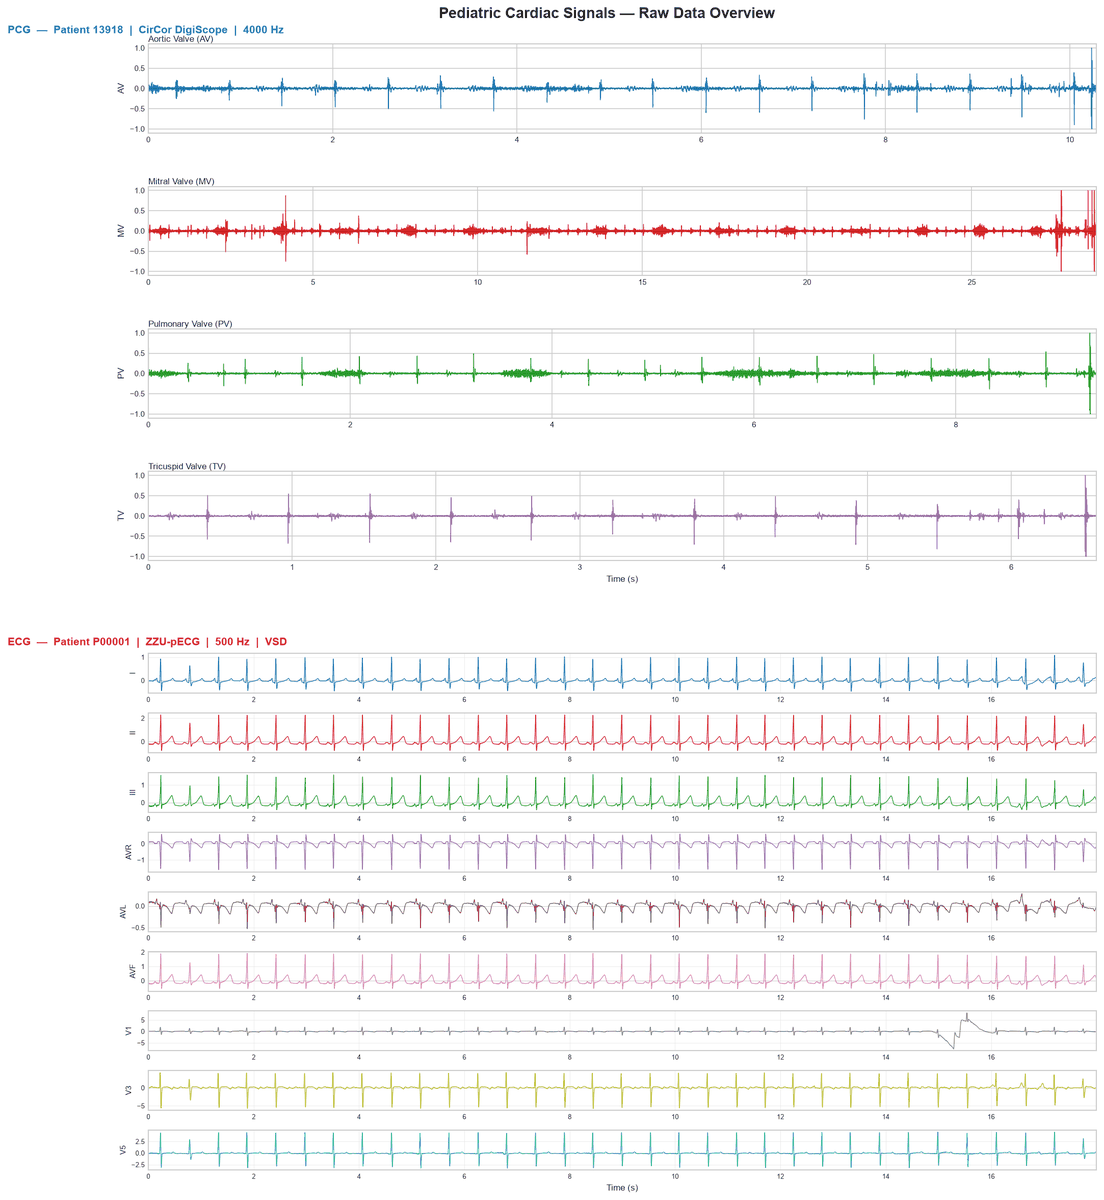
\includegraphics[width=0.92\linewidth]{report_images/combined_pcg_ecg_overview.png}
	\caption{Physiological overview of multi-modal pediatric cardiac screening signals: acoustic phonocardiogram audio waveforms and corresponding multi-lead electrocardiographic traces.}
	\label{fig:combined_pcg_ecg}
\end{figure}

\subsection{Phonocardiography (PCG)}
Phonocardiography refers to the high-fidelity acoustic transduction, amplification, and graphical recording of the acoustic sounds produced by the mechanical motion of the heart, the opening and closure of cardiac valves, and the turbulence of intracardiac blood flow \cite{leng2015phonocardiogram}. The normal physiological cardiac cycle produces two primary acoustic events: the first heart sound ($S_1$), generated by the closure of the atrioventricular (mitral and tricuspid) valves during the onset of ventricular systole; and the second heart sound ($S_2$), generated by the closure of the semilunar (aortic and pulmonary) valves at the termination of ventricular ejection. 

Structural cardiac anomalies, such as stenotic valves or septal perforations, generate high-velocity turbulent blood flow, producing audible acoustic vibrations termed \textit{cardiac murmurs}. Murmurs are clinically evaluated based on their acoustic timing (systolic, diastolic, or continuous), shape (crescendo-decrescendo, plateau, decrescendo), frequency spectrum (low, medium, high pitch), and anatomical auscultation location across the aortic, pulmonic, tricuspid, and mitral areas. Digital stethoscopes equipped with piezoelectric or electret microphone transducers enable electronic capture of PCG signals at sampling rates between 2 kHz and 4 kHz. Due to the portability, low hardware expense (frequently under \$100 to \$300 USD), and operational simplicity of modern digital stethoscopes, PCG constitutes the ideal frontline screening modality for primary health centres, community health workers, and rural mobile clinics \cite{oliveira2022circor}.

\subsection{Electrocardiography (ECG)}
Electrocardiography records the spatio-temporal bioelectric potentials generated by the cyclical depolarization and repolarization of myocardial tissue, measured via conductive electrodes affixed to standardized anatomical positions across the limbs and precordium \cite{kashou2020electrocardiogram}. Standard clinical setups employ 12-lead or 9-lead configurations, capturing orthogonal projections of the cardiac electrical vector ($V_1$ through $V_6$, Lead I, Lead II, Lead III, aVR, aVL, aVF). 

In pediatric medicine, ECG interpretation is uniquely challenging due to rapid developmental physiology. Neonates and infants exhibit marked physiological right ventricular dominance, shorter conduction intervals (PR interval, QRS duration), and resting heart rates that frequently exceed 120 to 160 beats per minute \cite{dicapua2019pediatric}. Pathological CHD phenotypes introduce pronounced electrical anomalies: large ventricular shunts produce biventricular hypertrophy with tall R waves and deep S waves; atrial defects generate right bundle branch block (RBBB) patterns and right axis deviation; and aortic coarctation manifests as severe left ventricular strain and voltage criteria for left ventricular hypertrophy. Multi-lead electrocardiographs are standard clinical equipment in secondary healthcare facilities, such as taluk hospitals, district general hospitals, and pediatric outpatient centers \cite{zheng202012}.

\subsection{Echocardiography (Echo)}
Transthoracic echocardiography is the clinical gold standard for the definitive anatomical and functional assessment of congenital heart defects. Echocardiography employs high-frequency ultrasound transducers (5 to 12 MHz in pediatric probes) to generate real-time two-dimensional (2D), M-mode, and Doppler visualizations of cardiac chambers, valves, septa, and great arterial anatomy \cite{lang2015recommendations}. 

Standard pediatric examination protocols acquire specific imaging windows, most notably the Apical Four-Chamber (AP4C) and Parasternal Short-Axis views. By capturing structural myocardial wall kinematics across the cardiac cycle, clinicians identify end-diastolic (ED) and end-systolic (ES) frames. Applying the biplane Simpson's method of discs enables clinicians to quantify Left Ventricular Internal Diameters, End-Diastolic Volumes (EDV), End-Systolic Volumes (ESV), and derive the global Left Ventricular Ejection Fraction (LVEF):
\begin{equation}
	\text{LVEF} = \frac{\text{EDV} - \text{ESV}}{\text{EDV}} \times 100\%
\end{equation}
In accordance with pediatric guidelines established by the American Society of Echocardiography (ASE), an LVEF below 55\% denotes compromised systolic pump performance, signifying severe myocardial dysfunction secondary to uncompensated volume or pressure overload \cite{lopez2010recommendations}. Transthoracic echocardiography suites are expensive (\$40,000 to \$150,000 USD) and necessitate years of specialized fellowship training to operate and interpret, confining this modality predominantly to advanced tertiary referral pediatric heart centres.

\begin{figure}[htbp]
	\centering
	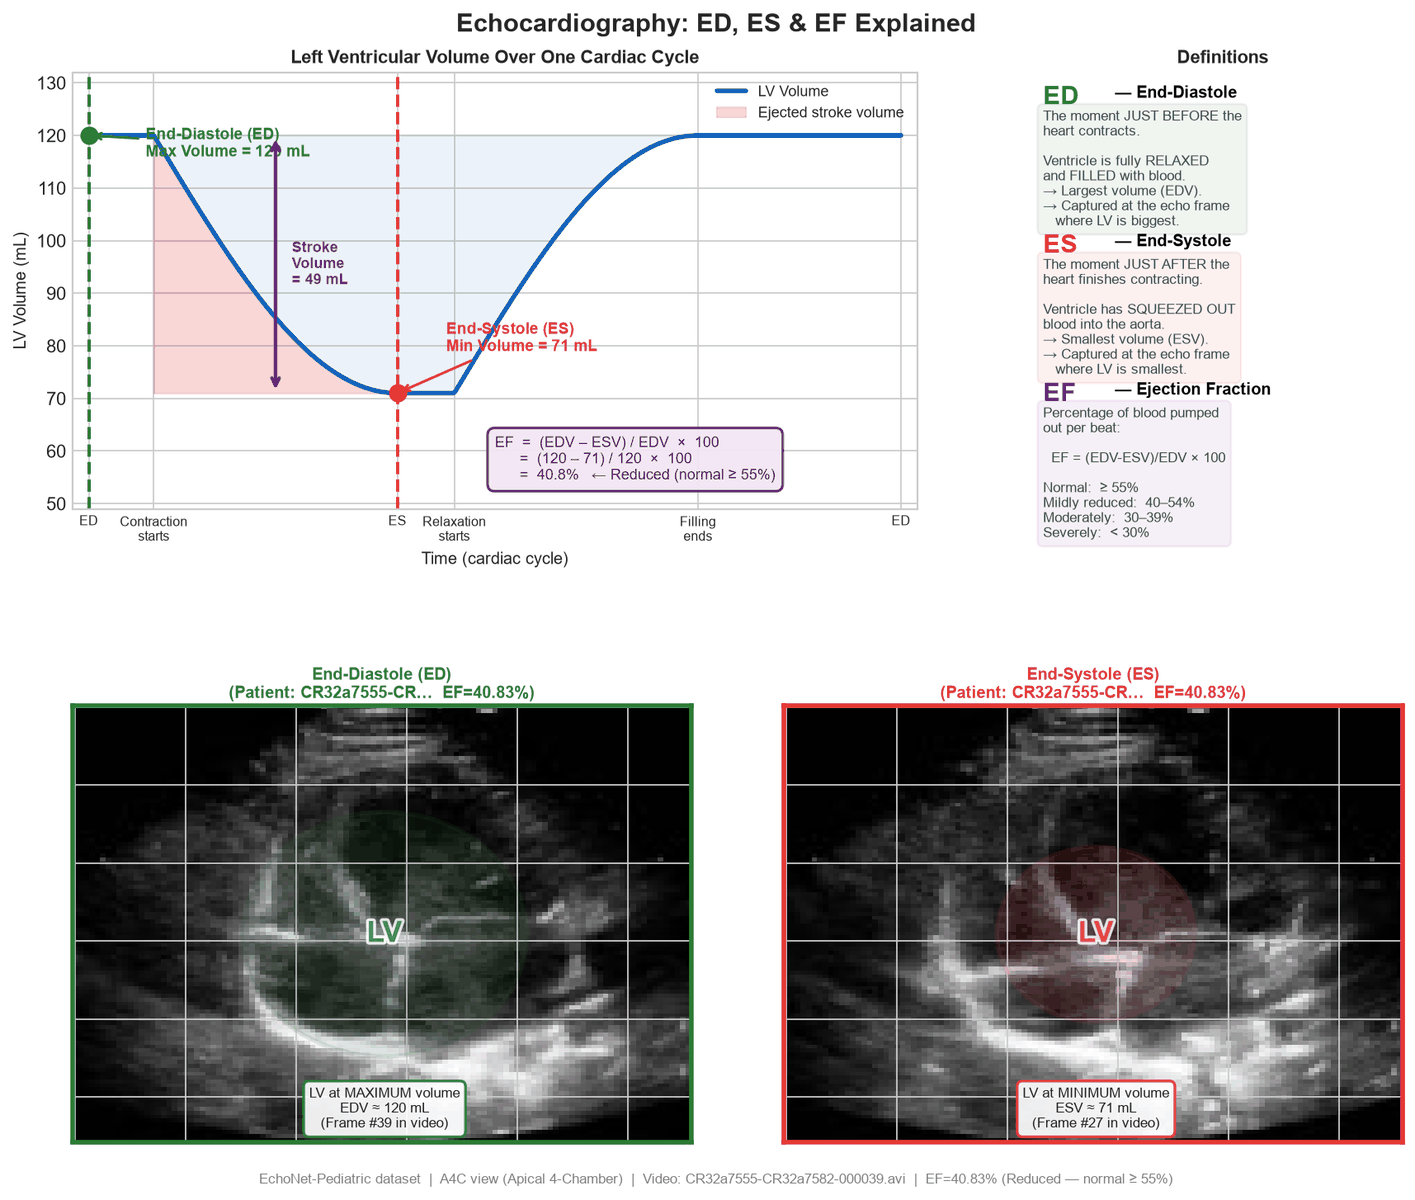
\includegraphics[width=0.88\linewidth]{report_images/echo_ed_es_ef_explained.png}
	\caption{Echocardiographic functional assessment: extraction of End-Diastolic (ED) and End-Systolic (ES) frame pairs and calculation of Left Ventricular Ejection Fraction (LVEF).}
	\label{fig:echo_explained}
\end{figure}


\section{THE MULTI-CENTER HEALTHCARE REALITY AND RESOURCE DISPARITY}

In realistic national and global healthcare systems, advanced diagnostic technologies are not distributed uniformly. Instead, healthcare delivery is structured as a tiered referral pyramid characterized by extreme equipment and expertise disparities across institutional tiers:
\begin{itemize}
	\item \textbf{Tier 1: Primary Healthcare Facilities and Rural Clinics (Hospital A).} These frontline outposts serve the vast majority of rural and low-income populations. They are staffed by general medical officers, nurses, or accredited community health workers. Diagnostic infrastructure is severely restricted; high-end imaging machines are entirely absent. The only objective cardiac diagnostic instrument available is a handheld electronic stethoscope capable of acquiring digital PCG heart sounds.
	\item \textbf{Tier 2: District General and Taluk Hospitals (Hospital B).} These secondary referral facilities serve medium-sized municipalities and regional districts. They possess dedicated diagnostic laboratories equipped with multi-lead diagnostic electrocardiograph machines (ECG) capable of recording 9-lead or 12-lead digital biosignals. However, they lack dedicated pediatric cardiologists and specialized pediatric ultrasound probes.
	\item \textbf{Tier 3: Specialized Tertiary Pediatric Heart Centres (Hospital C).} These elite academic medical centres feature specialized pediatric cardiology units equipped with state-of-the-art transthoracic echocardiography suites (Echo), cardiac magnetic resonance imaging, and pediatric catheterization laboratories.
\end{itemize}

A critical disconnect arises between where patients first present and where diagnostic expertise resides. Children born with life-threatening CHD initially present to Tier 1 rural clinics or Tier 2 district hospitals. If the attending primary healthcare practitioner fails to detect abnormal cardiac features, the child is sent home without specialist referral, frequently resulting in death before a tertiary centre is ever consulted. 

Automated artificial intelligence screening algorithms deployed at frontline clinics have the potential to bridge this gap by flagging abnormal cardiac status automatically. However, deep neural networks require massive, diverse training datasets to generalize effectively across heterogeneous patient cohorts.


\section{REGULATORY FRAMEWORKS AND CLINICAL DATA GOVERNANCE}

The conventional methodology for developing deep learning models in healthcare relies upon the centralized pooling of clinical data: medical centres export private patient records to a centralized cloud data warehouse, where a massive monolithic neural network is trained. In the context of multi-institutional pediatric medicine, this centralized approach is legally, ethically, and practically infeasible due to strict clinical data governance frameworks:
\begin{itemize}
	\item \textbf{Health Insurance Portability and Accountability Act (HIPAA):} In the United States, HIPAA's Privacy Rule strictly governs Protected Health Information (PHI). Exporting identifiable biosignals across institutional boundaries requires comprehensive de-identification protocols or explicit patient/guardian authorization, which is rarely attainable for large retrospective cohorts \cite{kaissis2020secure}.
	\item \textbf{General Data Protection Regulation (GDPR):} In the European Union, the GDPR classifies patient biometric and genetic data as ``special category data'' under Article 9. Strict data minimization principles and extraterritorial data transfer bans make cross-hospital or international data pooling legally precarious \cite{rumbold2017effect}.
	\item \textbf{Digital Personal Data Protection Act (DPDPA):} In India, emerging data privacy statutes impose stringent fiduciary responsibilities on health data fiduciaries, mandating localized processing and imposing severe financial penalties for unauthorized data exposure.
	\item \textbf{Institutional Review Boards (IRB) and Competitive Data Silos:} Beyond statutory regulations, individual hospital trusts and academic medical centres treat clinical datasets as proprietary intellectual property. Institutional risk aversion and competitive barriers routinely prevent hospitals from sharing raw clinical databases.
\end{itemize}

These regulatory and institutional barriers enforce strict \textit{data siloing}: patient data collected within Hospital A, Hospital B, and Hospital C must remain strictly resident on each institution's local secure storage servers.


\section{THE MACHINE LEARNING DILEMMA: CENTRALIZATION VS. ISLAND MODELS}

Faced with the impossibility of centralized data sharing, medical centres are forced to train ``island models''—deep neural networks trained strictly on each hospital's local patient dataset. However, isolated single-center training suffers from crippling theoretical and empirical pathologies:
\begin{enumerate}
	\item \textbf{Statistical Sample Scarcity and Overfitting:} Rare congenital defects (e.g., Tetralogy of Fallot, Truncus Arteriosus) manifest in small numbers within any single hospital's clinical intake. High-capacity neural networks trained on small local cohorts rapidly overfit to institutional idiosyncrasies, background acoustic noise, electrode impedances, or ultrasound transducer artifacts.
	\item \textbf{Severe Demographic Bias:} A model trained strictly on urban tertiary patients fails to generalize when deployed in rural clinics where patient demographics, nutritional baselines, maternal comorbidities, and prevalence rates differ drastically.
	\item \textbf{Narrow Diagnostic Perspective:} A model trained solely on PCG audio heart sounds can never learn the electrical conduction dynamics captured by ECG, nor can it comprehend the anatomical wall-motion geometry revealed by echocardiography.
\end{enumerate}

To overcome the pitfalls of isolated island models while respecting data privacy mandates, the machine learning community has turned to \textit{Federated Learning}.


\section{FEDERATED LEARNING AND THE CROSS-MODAL HETEROGENEITY BARRIER}

Federated Learning (FL), pioneered by McMahan et al. \cite{mcmahan2017communication}, is a decentralized machine learning paradigm wherein multiple distributed clients collaboratively optimize a global machine learning model under the coordination of a central server, without ever exchanging raw training data. 

In standard horizontal federated learning (e.g., the canonical \textbf{FedAvg} algorithm), the optimization objective across $K$ participating clients is defined as:
\begin{equation}
	\min_{w} F(w) = \sum_{k=1}^{K} \frac{n_k}{N} F_k(w)
\end{equation}
where $n_k$ is the number of samples at client $k$, $N = \sum_k n_k$, and $F_k(w) = \frac{1}{n_k} \sum_{i=1}^{n_k} \ell(f(x_i; w), y_i)$ is the local empirical loss function. In each communication round $t$:
\begin{enumerate}
	\item The central server broadcasts the current global parameter vector $w_t$ to all participating clients.
	\item Each client initializes its local model with $w_t$ and executes $E$ epochs of stochastic gradient descent on its private dataset:
	\begin{equation}
		w_{t+1}^k \leftarrow w_t - \eta \nabla F_k(w_t)
	\end{equation}
	\item Clients transmit their updated weight tensors $w_{t+1}^k$ (or weight deltas $\Delta w^k = w_{t+1}^k - w_t$) back to the central server.
	\item The central server performs coordinate-wise parameter averaging:
	\begin{equation}
		w_{t+1} = \sum_{k=1}^{K} \frac{n_k}{N} w_{t+1}^k
	\end{equation}
\end{enumerate}

While FedAvg and its proximal regularized variants (e.g., \textbf{FedProx} \cite{li2020federated}, \textbf{SCAFFOLD} \cite{karimireddy2020scaffold}) have achieved notable success in medical imaging domains where all institutions collect the same modality (e.g., brain MRI or chest X-rays), \textit{conventional federated learning completely breaks down in multi-modal healthcare ecosystems}.

The breakdown is structural and absolute:
\begin{enumerate}
	\item \textbf{Incompatible Input Spaces:} Hospital A processes 2D time-frequency audio spectrograms $x^A \in \mathbb{R}^{1 \times 64 \times 157}$; Hospital B processes 1D multi-channel electrical voltage time series $x^B \in \mathbb{R}^{9 \times 5000}$; and Hospital C processes 2D dual-frame spatial ultrasound tensors $x^C \in \mathbb{R}^{2 \times 112 \times 112}$.
	\item \textbf{Architectural Heterogeneity:} Processing these disparate signal spaces necessitates fundamentally different neural architectures. Hospital A requires a 2D audio convolutional network (PCGNet); Hospital B requires a 1D deep residual temporal network (ECGResNet); and Hospital C requires a 2D spatial feature extractor (EchoNet). 
	\item \textbf{Weight Averaging Impossibility:} Because the neural architectures share neither layer topologies, kernel dimensions, tensor ranks, nor parameter counts, coordinate-wise weight averaging ($\sum_k \frac{n_k}{N} w^k$) is mathematically undefined. There is no mathematical operation that can average a 1D convolution kernel of shape $[64, 9, 7]$ with a 2D convolution kernel of shape $[32, 1, 3, 3]$.
\end{enumerate}

To date, standard multimodal federated learning research has sidestepped this challenge by assuming that every client possesses all modalities simultaneously \cite{feng2023fedmultimodal}, or by requiring paired multi-modal datasets from the same patient cohort \cite{chen2023federated}. In pediatric cardiology, however, no such overlapping public datasets exist, and rural clinics will never possess echocardiogram suites. 

Therefore, a fundamental research question arises: \textit{How can hospitals with completely disjoint cardiac diagnostic modalities collaboratively train automated screening models without exchanging patient records or sharing neural network architectures?}


\section{PROBLEM STATEMENT}

This dissertation addresses the following clinically vital and mathematically challenging problem:

\begin{quote}
	\textit{``Given a decentralized healthcare consortium consisting of multiple independent hospitals, wherein each hospital possesses exclusively a single, structurally distinct cardiac screening modality (PCG audio at Hospital A, multi-lead ECG at Hospital B, and echocardiography frames at Hospital C), and wherein raw patient data cannot be exchanged due to statutory privacy mandates, design a federated learning framework that enables cross-modal knowledge transfer, achieves semantic representation alignment across incompatible latent spaces, and improves individual institutional screening performance over isolated single-center models without transmitting model parameters.''}
\end{quote}

\subsection{Formal Research Questions}
This investigation is structured around three foundational research questions:
\begin{itemize}
	\item \textbf{Research Question 1 (RQ1 - Representation Alignment):} How can semantically compatible representations of cardiac health status (Normal vs. Abnormal) be derived and aligned across neural networks operating on completely disparate physiological signal domains (acoustic audio, electrical conduction, and ultrasound imaging) without paired patient recordings?
	\item \textbf{Research Question 2 (RQ2 - Prototype Regularization):} Can class-level prototype vectors serve as an effective, privacy-preserving medium for cross-modal collaboration, and what mathematical loss formulations are required to prevent dimensional collapse and ensure stable convergence?
	\item \textbf{Research Question 3 (RQ3 - Clinical and Communication Efficiency):} Can a prototype-based cross-modal federated framework achieve screening efficacy (AUROC, Sensitivity, Specificity) matching or outperforming centralized or isolated baselines while operating under minimal network communication bandwidth suitable for rural clinical telematics?
\end{itemize}


\section{RESEARCH OBJECTIVES}

To answer these research questions, the project establishes the following specific objectives:
\begin{enumerate}
	\item \textbf{Development of the CrossFedProto Framework:} Formulate and implement \textbf{FedCardio}, a cross-modal federated prototype learning architecture that decouples local modality-specific feature extraction from global representation alignment using lightweight client-side projection heads.
	\item \textbf{Engineering Modality-Specific Feature Extractors:} Design, implement, and benchmark three specialized deep neural network architectures:
	\begin{itemize}
		\item \textit{PCGNet:} A 2D convolutional architecture processing log-mel-spectrogram representations of acoustic heart sounds.
		\item \textit{ECGResNet:} A 1D deep residual neural network capturing multi-lead cardiac electrophysiology.
		\item \textit{EchoNet:} A lightweight dual-channel convolutional network processing end-diastolic and end-systolic ultrasound frames.
	\end{itemize}
	\item \textbf{Mathematical Formulation of Dual Prototype Objectives:} Formulate a combined optimization objective that pairs directional hypersphere prototype alignment ($\mathcal{L}_{\text{proto}}$) with InfoNCE-style contrastive prototype separation ($\mathcal{L}_{\text{contrast}}$) to enforce tight intra-class clustering and wide inter-class separation across modalities.
	\item \textbf{Multi-Center Preprocessing and Curation Pipeline:} Develop automated, reproducible preprocessing pipelines for three benchmark pediatric datasets: the CirCor DigiScope Phonocardiogram Dataset ($n=11,162$ segments), the ZZU-pECG Pediatric Electrocardiogram Database ($n=14,190$ recordings), and the EchoNet-Pediatric Echocardiography Dataset ($n=3,258$ frame pairs).
	\item \textbf{Empirical Benchmarking and Ablation Studies:} Conduct rigorous empirical evaluations comparing CrossFedProto against isolated single-center baselines across clinical diagnostic metrics (AUROC, Sensitivity, Specificity, Accuracy, F1, F2, MCC) and analyze representation convergence via cosine distance tracking and t-SNE latent manifold visualization.
	\item \textbf{Explainable AI (XAI) Integration:} Integrate Gradient-Weighted Class Activation Mapping (Grad-CAM) to project model saliency back onto temporal acoustic heart sound intervals, providing clinicians with interpretable murmur localization.
	\item \textbf{Clinical Decision Support Software Platform:} Develop a production-ready, full-stack software application featuring a high-concurrency FastAPI asynchronous backend and an intuitive React/Vite web interface for interactive multi-modal pediatric screening and federated cluster orchestration.
\end{enumerate}


\section{SUMMARY OF NOVEL SCIENTIFIC CONTRIBUTIONS}

The key scientific and engineering contributions of this dissertation are summarized as follows:
\begin{enumerate}
	\item \textbf{Novel Cross-Modal Federated Prototype Learning Paradigm:} We propose CrossFedProto, the first federated learning framework specifically formulated for pediatric cardiac screening across completely disjoint physiological modalities (PCG, ECG, Echo) operating without paired multi-modal patient data or shared neural architectures.
	\item \textbf{Projection-Decoupled Alignment Architecture:} We introduce lightweight, client-side projection heads ($g_k: \mathbb{R}^{128} \rightarrow \mathbb{R}^{64}$) that project modality-specific latent embeddings onto a common unit hypersphere. This architectural decoupling preserves local inductive biases for classification while establishing a shared metric space for federated consensus.
	\item \textbf{Dual Prototype Loss with Contrastive Push-Pull Tension:} We design a composite training objective that combines class-weighted cosine prototype alignment with an InfoNCE contrastive anchor loss. We prove empirically that this combination eliminates prototype collapse, driving inter-client prototype cosine distance from 1.06 down to $< 0.001$.
	\item \textbf{Comprehensive Evaluation on 28,610 Pediatric Cohorts:} We execute extensive benchmarking across three major public pediatric cohorts, demonstrating that CrossFedProto matches or exceeds isolated single-center models, boosting ECG AUROC by +1.33\% (to 0.9594), surging PCG screening sensitivity by +6.84\% (to 89.46\%), and stabilizing Echo performance under severe 85:15 class imbalance.
	\item \textbf{Extreme Communication Efficiency:} We establish that CrossFedProto transmits only 128 floating-point values (512 bytes) per client per round, achieving an astounding 87,800-fold reduction in communication bandwidth compared to standard parameter-averaging FedAvg on the EchoNet backbone.
	\item \textbf{End-to-End Interpretable Clinical Deployment:} We deliver a clinically viable, explainable AI system featuring temporal Grad-CAM murmur localization and an interactive web-based diagnostic dashboard for multi-center federated deployment.
\end{enumerate}


\section{ORGANIZATION OF THE REPORT}

The remainder of this dissertation is organized as follows:
\begin{itemize}
	\item \textbf{Chapter 2 (Literature Review):} Provides a comprehensive critical review of prior scholarship spanning pediatric cardiac AI, phonocardiogram analysis, multi-lead ECG modeling, echocardiographic video assessment, federated learning paradigms, heterogeneous FL frameworks, and cross-modal alignment methods, culminating in a detailed comparative matrix and gap analysis.
	\item \textbf{Chapter 3 (Methodology / System Design):} Details the formal mathematical formulation of the FedCardio framework, the modality-specific neural architectures, the cross-modal projection mechanism, the square-root sample-weighted prototype aggregation algorithm, the dual prototype loss formulation, theoretical convergence dynamics, and privacy analysis.
	\item \textbf{Chapter 4 (Implementation):} Describes the experimental computational environment, dataset preprocessing and normalization pipelines, layer-by-layer neural network parameters, training hyperparameter configurations, the Grad-CAM explainability engine, and the architecture of the full-stack FastAPI and React/Vite clinical software platform.
	\item \textbf{Chapter 5 (Results and Discussion):} Presents exhaustive empirical results comparing CrossFedProto against single-center baselines, provides in-depth modality-specific clinical analyses, documents prototype convergence and t-SNE manifold alignment, details ablation studies, evaluates communication complexity, analyzes Youden-J decision thresholds, and examines clinical case studies.
	\item \textbf{Chapter 6 (Conclusion and Future Work):} Synthesizes the primary research findings, discusses clinical translational implications and technical limitations, and charts promising future avenues including multi-class defect classification, differential privacy integration, and edge-hardware deployment.
\end{itemize}


% ============================================================
% CHAPTER 2 - LITERATURE REVIEW
% ============================================================

\chapter{LITERATURE REVIEW}

\section{ARTIFICIAL INTELLIGENCE IN PHONOCARDIOGRAM ANALYSIS}

The automated acoustic analysis of phonocardiogram (PCG) signals has a rich history spanning classical digital signal processing, statistical machine learning, and modern deep neural networks. Early investigations focused primarily on the time-domain and frequency-domain segmentation of the fundamental heart sounds, $S_1$ and $S_2$. Schmidt et al. \cite{schmidt2010segmentation} developed duration-dependent Hidden Markov Models (HMM) capable of segmenting systolic and diastolic intervals by modeling the statistical state transitions between cardiac cycles. Springer et al. \cite{springer2015autoregressive} significantly advanced this paradigm by introducing an automated logistic regression-based hidden semi-Markov model (HSMM) incorporating homomorphic envelogram and wavelet features, establishing the benchmark segmentation framework utilized in the landmark 2016 PhysioNet/Computing in Cardiology Challenge \cite{clifford2016recent}.

While acoustic segmentation proved effective for clean recordings, the detection and grading of pathological murmurs under noisy, real-world clinical conditions remained a stubborn bottleneck. Classical approaches relied heavily upon handcrafted feature engineering, extracting Mel-Frequency Cepstral Coefficients (MFCC), discrete wavelet transform (DWT) subband energies, and spectral centroid dynamics, which were subsequently fed into shallow classifiers such as Support Vector Machines (SVM) or Random Forests \cite{leng2015phonocardiogram}. However, handcrafted features exhibited poor robustness against ambient acoustic environmental noise, crying pediatric subjects, respiratory sounds, and friction between the stethoscope chestpiece and patient skin.

The advent of deep learning revolutionized PCG interpretation. Rather than relying upon handcrafted acoustic heuristics, modern frameworks treat the 1D acoustic waveform as a 2D image by computing time-frequency representations via the Short-Time Fourier Transform (STFT) or Mel-scale filterbanks. Rubin et al. \cite{rubin2017recognizing} demonstrated that 2D Convolutional Neural Networks (CNNs) trained on log-mel-spectrograms achieved state-of-the-art performance in classifying normal versus abnormal heart sounds, demonstrating that convolutional kernels can autonomously discover spectro-temporal acoustic signatures characteristic of turbulent flow. 

The public release of the CirCor DigiScope Phonocardiogram Dataset \cite{oliveira2022circor} marked a pivotal watershed for pediatric-specific PCG analysis. Unlike earlier adult databases (e.g., the 2016 PhysioNet Challenge dataset), CirCor DigiScope focused explicitly upon pediatric patients screened during mass clinical campaigns in rural Brazil, providing real-world annotations of murmur presence, murmur timing, and overall clinical outcome. Winning solutions in the 2022 PhysioNet Challenge \cite{reyna2022heart} combined deep residual networks, ensemble 2D CNNs, and recurrent temporal aggregators. However, all published models on CirCor DigiScope operate within a strictly isolated, centralized learning regime; none have investigated how rural PCG acoustic models can collaboratively benefit from multi-lead ECG or echocardiographic data resident at secondary or tertiary urban hospitals.


\section{DEEP LEARNING FOR MULTI-LEAD ELECTROCARDIOGRAPHY}

Automated electrocardiogram (ECG) interpretation has served as an active domain of biomedical engineering for over five decades. Historically, computerized ECG algorithms relied upon the heuristic detection of fiducial points: identifying the onset, peak, and offset of P waves, QRS complexes, and T waves using derivative thresholding (e.g., the Pan-Tompkins algorithm \cite{pan1985real}) or wavelet multiresolution decomposition \cite{martinez2004wavelet}. Morphological features (QRS axis, QT dispersion, ST-segment elevation or depression) were subsequently mapped to clinical diagnostic rules. While highly effective for adult rhythm disorders (e.g., atrial fibrillation, ventricular tachycardia), rule-based algorithms frequently fail in pediatric populations due to the extreme physiological variability of cardiac conduction across developmental age brackets \cite{dicapua2019pediatric}.

In recent years, end-to-end deep learning architectures have demonstrated diagnostic accuracy rivaling expert cardiologists. In a landmark study, Ribeiro et al. \cite{ribeiro2020automatic} trained a deep 1D residual neural network (ResNet) on more than 2.3 million 12-lead ECG recordings from the Telehealth Network of Minas Gerais, achieving F1-scores exceeding 80\% across six common cardiac arrhythmias and outperforming resident medical professionals. Similarly, Hannun et al. \cite{hannun2019cardiologist} developed a 34-layer 1D convolutional network operating on single-lead ambulatory ECG patches, demonstrating dermatologist-level classification of twelve distinct rhythm categories. Attia et al. \cite{attia2019screening} made the groundbreaking discovery that deep 1D CNNs can detect asymptomatic left ventricular dysfunction (ejection fraction $\leq 35\%$) directly from surface 12-lead ECGs with an AUROC of 0.93, demonstrating that deep networks detect subtle electrophysiological signatures of structural myocardial disease that are imperceptible to human visual inspection.

Despite these dramatic breakthroughs in adult electrocardiology, deep learning investigations in \textit{pediatric} ECG analysis have been severely constrained by the lack of large, curated public datasets. Until recently, researchers were forced to fine-tune adult models or conduct studies on small, private single-institution cohorts comprising only a few hundred patients \cite{kashou2020electrocardiogram}. This severe data scarcity was definitively overcome with the publication of the ZZU-pECG database by Zheng et al. \cite{zheng2025zzu} in Nature \textit{Scientific Data}. Comprising 14,190 multi-lead pediatric ECG recordings from 11,643 children across 19 diagnostic categories, ZZU-pECG provides the first large-scale, open benchmark for pediatric cardiac electrophysiology. Nevertheless, existing deep learning models benchmarked on ZZU-pECG remain centralized, isolated, and disconnected from acoustic or structural imaging modalities.


\section{DEEP LEARNING IN ECHOCARDIOGRAPHY AND CARDIAC FUNCTION}

Echocardiography represents the most informative imaging modality in modern cardiology, offering dynamic structural visualization of cardiac anatomy, valve leaflets, and myocardial kinetics in real time. However, echocardiographic interpretation is notoriously plagued by high inter-observer and intra-observer variability: reported inter-cardiologist discrepancies in calculating Left Ventricular Ejection Fraction (LVEF) from 2D ultrasound video range between 8\% and 13\% \cite{lang2015recommendations}.

To standardize echocardiographic interpretation, deep learning researchers have pioneered computer vision architectures for automated view classification, anatomical segmentation, and functional quantification. Madani et al. \cite{madani2018fast} demonstrated that 2D CNNs can classify 15 standard echocardiographic views with 97.8\% accuracy, overcoming image quality variations. In a transformative study published in \textit{Nature}, Ouyang et al. \cite{ouyang2020video} introduced **EchoNet-Dynamic**, an end-to-end spatio-temporal video convolutional neural network (combining 3D ResNet convolutions with temporal pooling) trained on 10,030 apical-4-chamber echocardiogram videos. EchoNet-Dynamic achieved human-level segmentation of the left ventricle across cardiac cycles, predicting LVEF with a Mean Absolute Error (MAE) of 4.1\% and identifying heart failure with an AUROC of 0.93.

Extending these automated capabilities to pediatric cohorts, Lucile Packard Children's Hospital at Stanford published **EchoNet-Pediatric** \cite{ouyang2020video, he2023echonet}, comprising 7,643 labeled echocardiogram videos across 1,958 pediatric patients. EchoNet-Pediatric is acknowledged as the sole publicly available large-scale pediatric echocardiography dataset in existence today. The dataset contains expert clinical tracings identifying End-Diastolic (ED) and End-Systolic (ES) frames alongside biplane Simpson's rule ejection fraction annotations. However, utilizing EchoNet-Pediatric for automated screening introduces severe machine learning hurdles: the dataset exhibits extreme class imbalance (with over 85\% of subjects presenting normal systolic function) and high video dimensional complexity. 


\section{FEDERATED LEARNING PARADIGMS IN HEALTHCARE}

The imperative to preserve patient confidentiality while training high-capacity deep neural networks led to the rapid emergence of Federated Learning (FL) across healthcare informatics \cite{kaissis2020secure, xu2021federated}. In medical image computing, early consortia demonstrated that federated model training could approximate centralized training performance without data migration. Dayan et al. \cite{dayan2021federated} orchestrated the EXAMS federated initiative across 20 global hospitals, training an AI model that predicted oxygen therapy requirements in COVID-19 patients with an AUROC of 0.94, matching a centralized model trained on pooled patient records. Pati et al. \cite{pati2022federated} published the largest real-world healthcare federated study to date, uniting 71 international neuro-oncology institutions to train a deep 3D U-Net for glioblastoma boundary segmentation, demonstrating a 33\% improvement in boundary delineation over single-center models.

Despite these successes, standard federated learning algorithms suffer from significant theoretical failure modes when applied to non-IID (non-independent and identically distributed) client data:
\begin{enumerate}
	\item \textbf{Weight Divergence in FedAvg:} When local client data distributions $P_k(x, y)$ diverge significantly, local gradient updates $\nabla F_k(w)$ point in diametrically opposing directions. As proven by Li et al. \cite{li2020federated}, iterative local SGD causes client model weights $w^k$ to drift away from the optimal global consensus point, precipitating severe catastrophic forgetting and client drift.
	\item \textbf{Regularization Approaches (FedProx and SCAFFOLD):} To combat client drift, Li et al. \cite{li2020federated} introduced **FedProx**, which adds an $L_2$ proximal regularization term to the local objective:
	\begin{equation}
		\min_{w} F_k(w) + \frac{\mu}{2} \|w - w_t\|^2
	\end{equation}
	Karimireddy et al. \cite{karimireddy2020scaffold} introduced **SCAFFOLD**, utilizing client and server control variates to correct gradient direction variance.
\end{enumerate}

However, both FedProx and SCAFFOLD remain fundamentally bound to the \textit{homogeneous parameter assumption}: every client must execute identical neural network layers with identical parameter dimensions. They offer zero mathematical utility when client models possess incompatible architectures.


\section{HETEROGENEOUS FEDERATED LEARNING AND PROTOTYPE METHODS}

To dismantle the rigid constraint of architectural homogeneity, researchers have explored Heterogeneous Federated Learning. Three primary methodologies have emerged:
\begin{enumerate}
	\item \textbf{Knowledge Distillation (FedMD, FedDF):} Li and Wang \cite{li2019fedmd} proposed **FedMD**, wherein heterogeneous clients train unique local models and compute soft prediction logits on an auxiliary, publicly accessible unlabeled dataset. The server averages these soft logits, which clients subsequently utilize to distill consensus knowledge into their private backbones. Lin et al. \cite{lin2020ensemble} extended this with **FedDF** via ensemble distillation. However, distillation approaches fundamentally depend upon the existence of a high-quality, representative, and domain-relevant public dataset accessible to all clients. In cross-modal pediatric cardiology, no public dataset simultaneously containing paired PCG, ECG, and Echo signals exists, rendering distillation methods inapplicable.
	\item \textbf{Partial Model Sharing (Split Learning, FedPer):} Arivazhagan et al. \cite{arivazhagan2019federated} proposed **FedPer**, where clients share common base feature extractor layers while keeping top classification heads private. However, FedPer assumes that the base layers process identical input dimensions, which is impossible across 1D audio spectrograms, 1D ECG voltages, and 2D ultrasound frames.
	\item \textbf{Prototype-Based Federated Learning (FedProto, FedTGP):} Tan et al. \cite{tan2022fedproto} introduced **FedProto**, a pioneering paradigm that completely abandons parameter and gradient exchange. Instead of communicating model weights, clients compute and transmit \textit{class prototype vectors}—defined as the mathematical mean of penultimate-layer latent embeddings for each class:
	\begin{equation}
		p_k^c = \frac{1}{|D_k^c|} \sum_{i \in D_k^c} f_k(x_i)
	\end{equation}
	The central server averages these local prototypes into global prototypes $P^c = \sum_k \frac{n_k^c}{\sum_j n_j^c} p_k^c$, which are broadcast back to clients to serve as $L_2$ metric regularization targets during local training. Dai et al. \cite{dai2023tackling} proposed **FedNH**, introducing learnable class prototypes with prototype orthogonality, while Zhang et al. \cite{zhang2024fedtgp} developed **FedTGP**, employing adaptive-margin contrastive global prototypes.
\end{enumerate}

Crucially, however, all prior prototype FL literature (FedProto, FedNH, FedTGP) evaluated their frameworks strictly on \textit{uni-modal datasets} (e.g., partitioned MNIST, CIFAR-10, or DomainNet) where clients processed the same data domain (images) using different CNN backbones (e.g., ResNet-18 vs. MobileNet vs. ShuffleNet). None investigated the behavior of prototype learning when clients operate on \textit{completely disjoint physical modalities}.


\section{CROSS-MODAL REPRESENTATION LEARNING AND THE SEMANTIC GAP}

Mapping disparate physiological and sensory modalities into a unified semantic coordinate system is the central objective of Cross-Modal Representation Learning \cite{baltruvsaitis2018multimodal}. In centralized multi-modal machine learning, contrastive learning paradigms have achieved extraordinary breakthroughs. Radford et al. \cite{radford2021learning} introduced **CLIP** (Contrastive Language-Image Pretraining), training independent visual and textual transformers to maximize the cosine similarity of paired image-text embeddings across a batch via symmetric InfoNCE loss. In the medical domain, Zhang et al. \cite{zhang2022contrastive} introduced **ConVIRT**, successfully aligning chest X-ray images with unstructured clinical radiology reports.

In the federated sphere, multimodal research has gained traction through recent benchmarks such as **FedMultimodal** \cite{feng2023fedmultimodal}. Le et al. \cite{le2024multimodal} proposed **MFCPL** (Multimodal Federated Contrastive Prototype Learning), utilizing contrastive prototype objectives for medical image segmentation across clinical sites. 

However, existing multimodal FL literature universally relies upon two restrictive assumptions:
\begin{enumerate}
	\item \textbf{Modality Overlap:} Participating clients possess overlapping subsets of modalities (e.g., Client 1 has Modality A+B, Client 2 has B+C).
	\item \textbf{Paired Instances:} Multimodal data is collected concurrently from identical patient encounters, enabling direct paired contrastive optimization.
\end{enumerate}

In the real-world healthcare scenario addressed in this dissertation, both assumptions are violated: Hospital A has \textit{only} PCG, Hospital B has \textit{only} ECG, and Hospital C has \textit{only} Echo. There is zero modality overlap, and zero paired patient data. Naive prototype averaging across such disjoint native embedding spaces fails catastrophically because the latent coordinate systems of unaligned models possess completely arbitrary semantic bases—a critical challenge termed the \textit{Semantic Disconnection Problem} \cite{le2024multimodal}.


\section{EXPLAINABLE AI (XAI) IN CLINICAL DECISION SUPPORT}

The black-box nature of deep neural networks represents a severe impediment to clinical translation and regulatory approval by agencies such as the US Food and Drug Administration (FDA) and the European Medicines Agency (EMA) \cite{amann2020explainability}. Clinicians cannot responsibly base triage or surgical referral decisions upon an opaque probability score generated by millions of uninterpretable weights. 

To instill clinical trust, Explainable AI (XAI) frameworks seek to render deep network decisions transparent. Selvaraju et al. \cite{selvaraju2017grad} formulated Gradient-Weighted Class Activation Mapping (**Grad-CAM**), which computes the gradients of a target class score $y^c$ with respect to the feature activation maps $A^k$ of the final convolutional layer:
\begin{equation}
	\alpha_k^c = \frac{1}{Z} \sum_{i} \sum_{j} \frac{\partial y^c}{\partial A_{i, j}^k}
\end{equation}
The coarse heat-map localization is obtained via a rectified linear combination:
\begin{equation}
	L_{\text{Grad-CAM}}^c = \text{ReLU}\left(\sum_k \alpha_k^c A^k\right)
\end{equation}
While Grad-CAM is standard in natural 2D medical computer vision (e.g., highlighting pneumonia lesions on chest radiographs), its adaptation to time-frequency acoustic phonocardiograms requires projecting spatial-frequency activations back onto 1D temporal intervals to align with clinical auscultation phases ($S_1$, systole, $S_2$, diastole). Providing automated temporal murmur localization transforms an algorithmic screening flag into an actionable diagnostic aid for primary care physicians.


\section{COMPARATIVE LITERATURE MATRIX}

To explicitly contextualize the position of this dissertation within the broader research landscape, Table \ref{tab:lit_matrix} presents a rigorous comparative analysis of 12 landmark benchmark publications across federated learning, multimodal diagnostics, and cardiac artificial intelligence.

\begin{table}[htbp]
	\centering
	\caption{Comparative Literature Matrix: Benchmarking Existing State-of-the-Art against FedCardio}
	\label{tab:lit_matrix}
	\resizebox{\linewidth}{!}{%
	\begin{tabular}{|l|c|c|c|c|c|c|c|}
		\hline
		\textbf{Author \& Year} & \textbf{Target Modality} & \textbf{FL Paradigm} & \textbf{Arch. Agnostic?} & \textbf{Disjoint Modalities?} & \textbf{No Shared Data?} & \textbf{XAI Engine?} & \textbf{Pediatric Focus?} \\
		\hline
		McMahan et al. (2017) \cite{mcmahan2017communication} & General / Text & Weight Averaging (FedAvg) & No & No & Yes & No & No \\
		Li et al. (2020) \cite{li2020federated} & General Image & Proximal Regularization (FedProx) & No & No & Yes & No & No \\
		Ribeiro et al. (2020) \cite{ribeiro2020automatic} & 12-lead ECG & Centralized Deep ResNet & N/A & No & No & No & No \\
		Ouyang et al. (2020) \cite{ouyang2020video} & Echo Video & Centralized Video ResNet & N/A & No & No & Yes & No \\
		Dayan et al. (2021) \cite{dayan2021federated} & Chest X-ray & Weight Averaging (FedAvg) & No & No & Yes & No & No \\
		Tan et al. (2022) \cite{tan2022fedproto} & Single-Domain Vision & Prototype Averaging (FedProto) & Yes & No & Yes & No & No \\
		Oliveira et al. (2022) \cite{oliveira2022circor} & PCG Audio & Centralized 2D CNN Ensemble & N/A & No & No & No & Yes \\
		Feng et al. (2023) \cite{feng2023fedmultimodal} & Multimodal Benchmark & Overlapping FL & No & No & Yes & No & No \\
		Zhang et al. (2024) \cite{zhang2024fedtgp} & Single-Domain Vision & Trainable Prototypes (FedTGP) & Yes & No & Yes & No & No \\
		Le et al. (2024) \cite{le2024multimodal} & Multimodal Imaging & Contrastive Prototypes (MFCPL) & Yes & No (Overlapping) & Yes & No & No \\
		Zheng et al. (2025) \cite{zheng2025zzu} & Pediatric ECG & Centralized Benchmark & N/A & No & No & No & Yes \\
		\hline
		\textbf{FedCardio (This Work)} & \textbf{PCG + ECG + Echo} & \textbf{CrossFedProto} & \textbf{Yes} & \textbf{Yes (100\% Disjoint)} & \textbf{Yes} & \textbf{Yes (Grad-CAM)} & \textbf{Yes} \\
		\hline
	\end{tabular}%
	}
\end{table}


\section{IDENTIFIED RESEARCH GAPS AND MOTIVATION}

The comprehensive critical analysis of contemporary literature exposes three fundamental, unaddressed research gaps:
\begin{enumerate}
	\item \textbf{The Cross-Modal Disjoint Modality Void:} Existing federated prototype frameworks (FedProto, FedTGP) were engineered under the foundational assumption that clients observe the same physical domain. No methodology exists to enable federated collaboration when participating hospitals possess completely disjoint, non-overlapping sensory modalities without paired multi-modal samples.
	\item \textbf{The Prototype Collapse Vulnerability in Disparate Metric Spaces:} When $L_2$ prototype regularization is applied across heterogeneous encoders with disparate inductive biases, models frequently suffer from catastrophic prototype collapse, wherein positive and negative class representations collapse together on the latent manifold, severely degrading clinical sensitivity.
	\item \textbf{Absence of Privacy-Preserving Collaborative Systems for Pediatric Screening:} While pediatric congenital heart disease represents a devastating global health crisis, no privacy-preserving federated screening framework has been formulated to unite frontline rural clinics (PCG), secondary district hospitals (ECG), and advanced tertiary heart centres (Echo) into an integrated clinical decision support network.
\end{enumerate}

These critical gaps provide the precise scientific and clinical motivation for \textbf{FedCardio}, presented in Chapter 3.


% ============================================================
% CHAPTER 3 - METHODOLOGY / SYSTEM DESIGN
% ============================================================

\chapter{METHODOLOGY / SYSTEM DESIGN}

\section{MATHEMATICAL PROBLEM FORMULATION}

We formalize the decentralized cross-modal pediatric cardiac screening problem across a consortium of $K$ independent hospital institutions. Let $\mathcal{K} = \{1, 2, \dots, K\}$ denote the set of participating hospital clients. In our clinical framework, $K = 3$, representing the tiered healthcare hierarchy:
\begin{itemize}
	\item Client $k=1$ represents \textbf{Hospital A} (Rural Primary Health Clinic), possessing private dataset $\mathcal{D}_1$ composed of Phonocardiogram (PCG) acoustic recordings.
	\item Client $k=2$ represents \textbf{Hospital B} (District General Hospital), possessing private dataset $\mathcal{D}_2$ composed of multi-lead Electrocardiogram (ECG) voltage signals.
	\item Client $k=3$ represents \textbf{Hospital C} (Tertiary Children's Heart Centre), possessing private dataset $\mathcal{D}_3$ composed of Transthoracic Echocardiogram (Echo) video frame pairs.
\end{itemize}

Each client $k \in \mathcal{K}$ holds a private dataset $\mathcal{D}_k = \{(x_i^k, y_i^k)\}_{i=1}^{n_k}$, where $n_k = |\mathcal{D}_k|$ denotes the sample size at institution $k$. Crucially:
\begin{itemize}
	\item The input feature spaces are completely disjoint: $x_i^k \in \mathcal{X}_k$, where $\mathcal{X}_1 \neq \mathcal{X}_2 \neq \mathcal{X}_3$. Specifically, $\mathcal{X}_1 \subset \mathbb{R}^{1 \times F \times T}$ (time-frequency spectrograms), $\mathcal{X}_2 \subset \mathbb{R}^{C \times L}$ (multi-channel temporal series), and $\mathcal{X}_3 \subset \mathbb{R}^{2 \times H \times W}$ (dual-frame structural images).
	\item The label space is shared and globally unified: $y_i^k \in \mathcal{Y} = \{0, 1\}$, where $y=0$ denotes a **Normal** cardiac status (benign physiology, no intervention needed), and $y=1$ denotes an **Abnormal** cardiac status (presence of congenital defect or hemodynamic dysfunction, mandating specialist pediatric cardiology referral).
	\item There is zero patient overlap across cohorts: $\mathcal{D}_1 \cap \mathcal{D}_2 \cap \mathcal{D}_3 = \emptyset$.
\end{itemize}

Each hospital operates a local neural network composed of two primary functional components:
\begin{enumerate}
	\item A modality-specific feature encoder $f_k(\cdot; \theta_k): \mathcal{X}_k \rightarrow \mathbb{R}^{d}$, parametrized by weights $\theta_k$, which maps raw physiological signals into a $d$-dimensional native latent embedding space ($d = 128$).
	\item A local classification head $h_k(\cdot; \phi_k): \mathbb{R}^{d} \rightarrow \mathbb{R}^{|\mathcal{Y}|}$, parametrized by weights $\phi_k$, which produces class prediction logits for local patient inference.
\end{enumerate}

Because $\theta_1, \theta_2, \theta_3$ represent fundamentally different tensor dimensions and layer topologies, direct parameter aggregation $\sum_k w_k \theta_k$ is strictly impossible.

\begin{figure}[htbp]
	\centering
	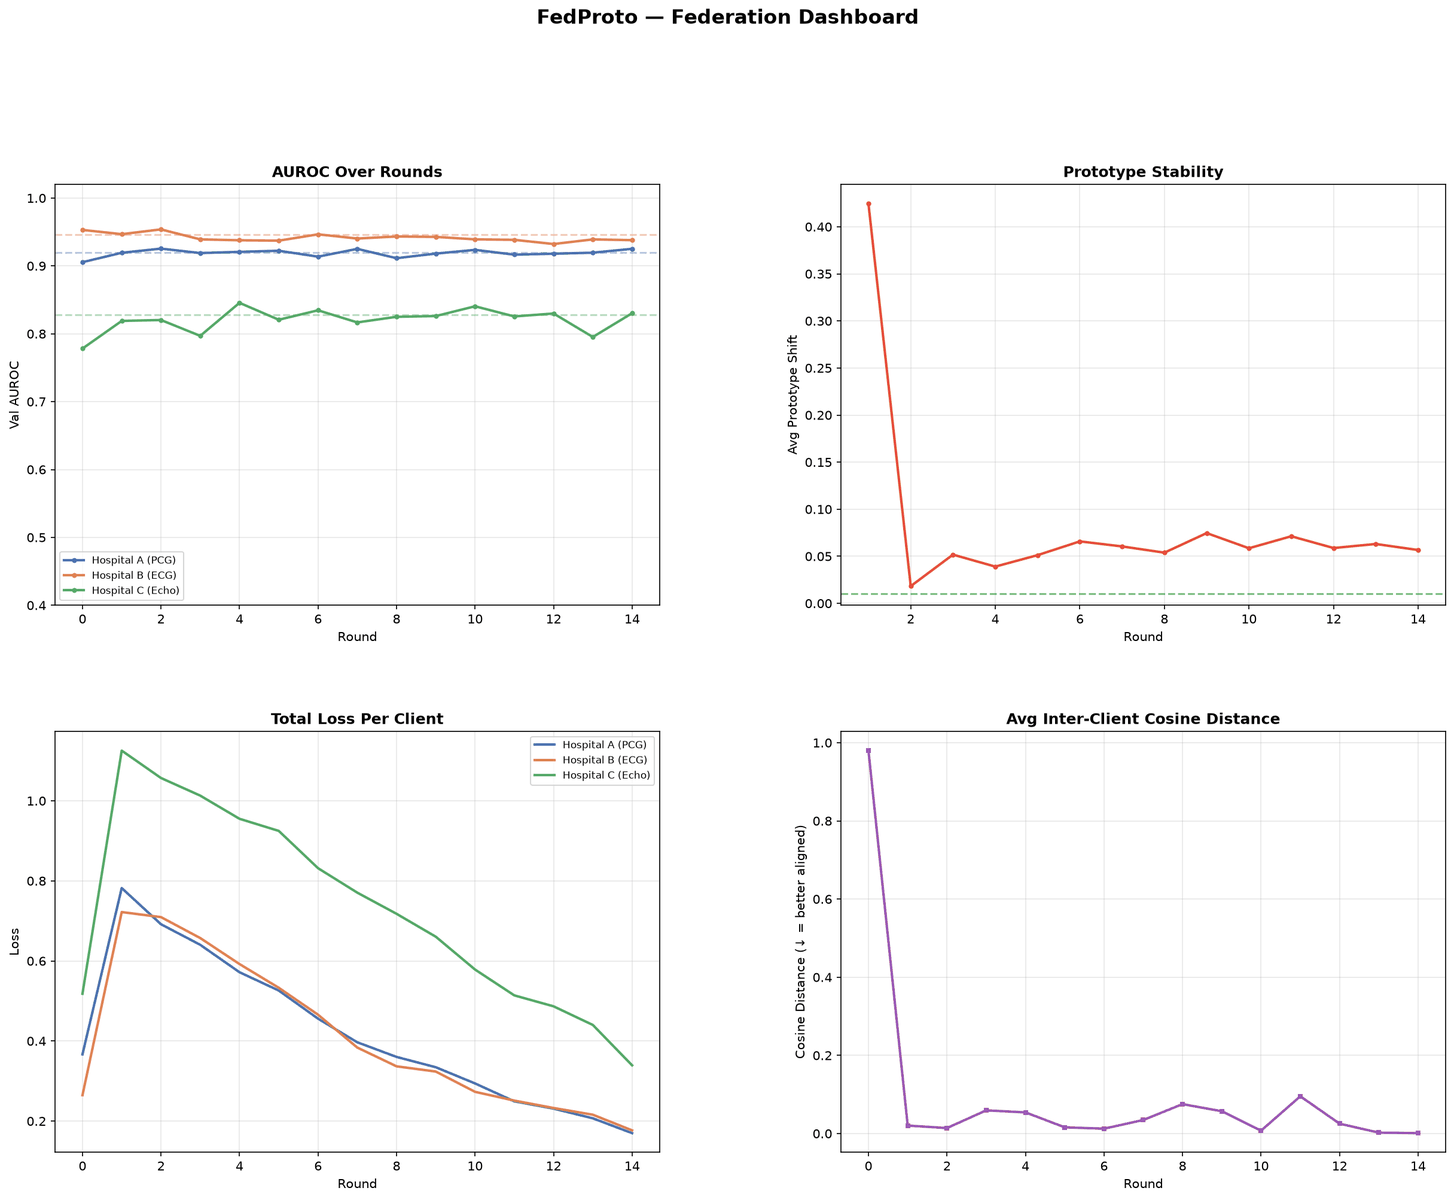
\includegraphics[width=0.95\linewidth]{report_images/federation_dashboard.png}
	\caption{FedCardio System Architecture: Decentralized hospital clients (PCG, ECG, Echo) training locally with projection heads, communicating solely class prototype vectors to the central aggregation server.}
	\label{fig:fedcardio_system}
\end{figure}


\section{CLIENT-LEVEL MODALITY ENCODERS}

To optimize local diagnostic performance while preserving feature expressiveness, we engineer three distinct modality-specific neural architectures, illustrated schematically below.

\subsection{PCGNet: 2D Convolutional Spectrogram Encoder (Hospital A)}
Hospital A processes acoustic phonocardiograms converted into 64-bin log-mel-spectrograms. The input tensor is $x \in \mathbb{R}^{1 \times 64 \times 157}$, representing 5 seconds of heart sound audio sampled at 4 kHz with an FFT window length of $N_{\text{FFT}} = 512$ and hop size $H = 128$.

PCGNet processes the spectrogram via three sequential convolutional blocks followed by adaptive pooling. Each block applies a 2D convolution, Batch Normalization, ReLU activation, and 2D Max Pooling:
\begin{align}
	H_1 &= \text{MaxPool}_{2 \times 2}\left(\text{ReLU}\left(\text{BN}\left(\text{Conv2D}_{1 \rightarrow 32, 3 \times 3}(x)\right)\right)\right) \in \mathbb{R}^{32 \times 32 \times 78} \\
	H_2 &= \text{MaxPool}_{2 \times 2}\left(\text{ReLU}\left(\text{BN}\left(\text{Conv2D}_{32 \rightarrow 64, 3 \times 3}(H_1)\right)\right)\right) \in \mathbb{R}^{64 \times 16 \times 39} \\
	H_3 &= \text{MaxPool}_{2 \times 2}\left(\text{ReLU}\left(\text{BN}\left(\text{Conv2D}_{64 \rightarrow 128, 3 \times 3}(H_2)\right)\right)\right) \in \mathbb{R}^{128 \times 8 \times 19}
\end{align}
The feature tensor $H_3$ is downsampled using Adaptive Average Pooling to a fixed spatial grid:
\begin{equation}
	H_{\text{pool}} = \text{AdaptiveAvgPool2D}_{4 \times 4}(H_3) \in \mathbb{R}^{128 \times 4 \times 4}
\end{equation}
Flattening $H_{\text{pool}}$ yields a 2,048-dimensional vector, which is projected through a fully connected dense layer and dropout ($p=0.3$) to produce the native 128-dimensional embedding:
\begin{equation}
	e_{\text{PCG}} = f_1(x; \theta_1) = \text{Dropout}_{0.3}\left(\text{Linear}_{2048 \rightarrow 128}(\text{vec}(H_{\text{pool}}))\right) \in \mathbb{R}^{128}
\end{equation}
The local classifier $h_1$ maps $e_{\text{PCG}}$ to binary logits: $\hat{y} = \text{Linear}_{128 \rightarrow 2}(e_{\text{PCG}})$. Total PCGNet parameters: 355,426.

\subsection{ECGResNet: 1D Deep Residual Temporal Encoder (Hospital B)}
Hospital B processes 9-lead electrocardiogram signals standardized to a 10-second duration sampled at 500 Hz: $x \in \mathbb{R}^{9 \times 5000}$. To capture multi-lead electrical conduction morphology while preventing vanishing gradients across temporal depth, ECGResNet employs a 1D deep residual network.

The network initiates with an input convolutional stem:
\begin{equation}
	Z_0 = \text{ReLU}\left(\text{BN}\left(\text{Conv1D}_{9 \rightarrow 32, k=7, s=2, p=3}(x)\right)\right) \in \mathbb{R}^{32 \times 2500}
\end{equation}
This is followed by five residual blocks with increasing channel width ($\{32, 64, 128, 256, 256\}$) and strided downsampling ($s=2$ at transitions). Each residual block executes:
\begin{equation}
	\mathcal{F}(Z_{l-1}) = \text{BN}\left(\text{Conv1D}\left(\text{ReLU}\left(\text{BN}\left(\text{Conv1D}(Z_{l-1})\right)\right)\right)\right)
\end{equation}
\begin{equation}
	Z_l = \text{ReLU}\left(\mathcal{F}(Z_{l-1}) + \mathcal{W}_s(Z_{l-1})\right)
\end{equation}
where $\mathcal{W}_s$ denotes a $1 \times 1$ convolutional shortcut when spatial downsampling occurs. Following Block 5 ($Z_5 \in \mathbb{R}^{256 \times 78}$), global temporal representation is extracted via 1D Global Average Pooling:
\begin{equation}
	Z_{\text{gap}} = \text{GAP1D}(Z_5) = \frac{1}{T}\sum_{t=1}^{T} Z_5[:, t] \in \mathbb{R}^{256}
\end{equation}
A dense linear projection maps $Z_{\text{gap}}$ to the native 128-dimensional embedding:
\begin{equation}
	e_{\text{ECG}} = f_2(x; \theta_2) = \text{Dropout}_{0.3}\left(\text{Linear}_{256 \rightarrow 128}(Z_{\text{gap}})\right) \in \mathbb{R}^{128}
\end{equation}
The local classifier $h_2$ maps $e_{\text{ECG}}$ to binary logits: $\hat{y} = \text{Linear}_{128 \rightarrow 2}(e_{\text{ECG}})$. Total ECGResNet parameters: 1,970,978.

\subsection{EchoNet: Bi-Chamber Dual-Frame Ultrasound Encoder (Hospital C)}
Hospital C processes transthoracic echocardiogram video frames. Rather than processing full 3D video volumes which induces severe computational latency and overfits small cohorts, EchoNet takes as input the paired End-Diastolic (ED) and End-Systolic (ES) grayscale frames resized to $112 \times 112$: $x \in \mathbb{R}^{2 \times 112 \times 112}$. Stacking ED and ES along the channel axis permits the 2D convolutions to directly learn spatial displacement differences (wall motion velocity and chamber contraction) between ventricular filling and ejection.

EchoNet employs a lightweight 4-block convolutional backbone replacing heavy pre-trained backbones:
\begin{align}
	U_1 &= \text{MaxPool}_{2 \times 2}\left(\text{ReLU}\left(\text{BN}\left(\text{Conv2D}_{2 \rightarrow 32, 3 \times 3}(x)\right)\right)\right) \in \mathbb{R}^{32 \times 56 \times 56} \\
	U_2 &= \text{MaxPool}_{2 \times 2}\left(\text{ReLU}\left(\text{BN}\left(\text{Conv2D}_{32 \rightarrow 64, 3 \times 3}(U_1)\right)\right)\right) \in \mathbb{R}^{64 \times 28 \times 28} \\
	U_3 &= \text{MaxPool}_{2 \times 2}\left(\text{ReLU}\left(\text{BN}\left(\text{Conv2D}_{64 \rightarrow 128, 3 \times 3}(U_2)\right)\right)\right) \in \mathbb{R}^{128 \times 14 \times 14} \\
	U_4 &= \text{MaxPool}_{2 \times 2}\left(\text{ReLU}\left(\text{BN}\left(\text{Conv2D}_{128 \rightarrow 256, 3 \times 3}(U_3)\right)\right)\right) \in \mathbb{R}^{256 \times 7 \times 7}
\end{align}
Applying 2D Global Average Pooling yields:
\begin{equation}
	U_{\text{gap}} = \text{GAP2D}(U_4) \in \mathbb{R}^{256}
\end{equation}
Dense transformation produces the native 128-dimensional embedding:
\begin{equation}
	e_{\text{Echo}} = f_3(x; \theta_3) = \text{Dropout}_{0.3}\left(\text{Linear}_{256 \rightarrow 128}(U_{\text{gap}})\right) \in \mathbb{R}^{128}
\end{equation}
Local classifier $h_3$ produces output logits: $\hat{y} = \text{Linear}_{128 \rightarrow 2}(e_{\text{Echo}})$. Total EchoNet parameters: 422,178.


\section{THE CROSS-MODAL EMBEDDING ALIGNMENT PROBLEM}

Even though all three client encoders output native latent vectors of identical mathematical dimension ($d = 128$), \textbf{these vectors cannot be averaged}. 

Mathematically, the native latent embedding space $\mathbb{R}^d$ of each neural network represents an internal coordinate frame whose basis vectors are determined arbitrarily by random parameter initialization and modality-specific stochastic gradient descent. For example:
\begin{itemize}
	\item In PCGNet, dimension $j$ might encode the high-frequency acoustic energy of an early systolic ejection murmur.
	\item In ECGResNet, dimension $j$ might encode the ST-segment elevation in precordial lead $V_2$.
	\item In EchoNet, dimension $j$ might encode the end-systolic apical wall thickness.
\end{itemize}

Averaging vectors across these unaligned native coordinate systems is semantically meaningless—analogous to averaging the ASCII numerical codes of an English sentence and a Mandarin sentence. Naive FedProto executed directly on native embeddings fails to achieve semantic consensus, resulting in destructive gradient interference.


\section{CROSSFEDPROTO: LEARNABLE PROJECTION HEADS}

To bridge this semantic chasm without compromising local model discriminability, FedCardio introduces a \textbf{Lightweight Learnable Projection Head} $g_k(\cdot; \psi_k)$ on each client, mapping from the native embedding space $\mathbb{R}^d$ into a shared, lower-dimensional alignment space $\mathbb{R}^p$ ($d = 128, p = 64$):
\begin{equation}
	z_i^k = g_k(e_i^k; \psi_k) = \text{LayerNorm}\left(\text{ReLU}\left(\mathcal{W}_{\text{proj}}^k e_i^k + b_{\text{proj}}^k\right)\right) \in \mathbb{R}^{64}
\end{equation}
where $\mathcal{W}_{\text{proj}}^k \in \mathbb{R}^{64 \times 128}$ and $b_{\text{proj}}^k \in \mathbb{R}^{64}$. Each projection head adds merely $128 \times 64 + 64 = 8,256$ parameters, imposing virtually zero computational overhead.

Crucially, projected embeddings are mapped onto the unit hypersphere $\mathbb{S}^{p-1}$ via $L_2$ normalization:
\begin{equation}
	\bar{z}_i^k = \frac{z_i^k}{\|z_i^k\|_2} = \frac{g_k(f_k(x_i^k))}{\|g_k(f_k(x_i^k))\|_2}
\end{equation}

\subsection{Architectural Decoupling Rationale}
This architectural decoupling is of paramount theoretical significance:
\begin{enumerate}
	\item \textbf{Preservation of Local Discriminative Inductive Bias:} The primary classification head $h_k$ continues to operate directly on the 128-dimensional native embedding $e_i^k$. Local screening performance is never constrained by the global alignment subspace.
	\item \textbf{Translation into Shared Semantic Lingua Franca:} The projection head $g_k$ acts as an autonomous neural translator. It learns to rotate and compress the client's internal diagnostic features such that shared pathological concepts (Normal vs. Abnormal) map to identical coordinates on the unit hypersphere $\mathbb{S}^{63}$.
\end{enumerate}


\section{FEDERATED PROTOTYPE COMPUTATION AND AGGREGATION}

Rather than transmitting neural network weights $\theta_k$ or private sample embeddings $z_i^k$, FedCardio communicates exclusively class prototype vectors.

\subsection{Client-Side Prototype Extraction}
At the conclusion of each local training epoch, client $k$ partitions its local training cohort $\mathcal{D}_k$ by ground-truth class label $c \in \{0, 1\}$. The local class prototype $p_k^c$ is computed as the normalized centroid of all projected embeddings belonging to class $c$:
\begin{equation}
	p_k^c = \frac{1}{|\mathcal{D}_k^c|} \sum_{i \in \mathcal{D}_k^c} \bar{z}_i^k = \frac{1}{n_k^c} \sum_{i: y_i^k = c} \frac{g_k(f_k(x_i^k))}{\|g_k(f_k(x_i^k))\|_2} \in \mathbb{R}^{64}
\end{equation}
Each client transmits exactly two 64-dimensional vectors ($p_k^0$ and $p_k^1$) alongside its class sample counts ($n_k^0$ and $n_k^1$) to the central aggregation server.

\subsection{Server-Side Square-Root Sample-Weighted Aggregation}
In conventional FedProto, server aggregation weights each client linearly by sample size: $w_k = n_k^c / \sum_j n_j^c$. In multi-center healthcare, however, linear weighting induces severe \textit{client domination}: Hospital B (ECG, $n=14,190$) would completely overwhelm Hospital C (Echo, $n=3,258$), forcing the global prototype to mirror ECG features while ignoring echocardiographic geometry.

To ensure equitable cross-modal representation, the FedCardio server executes **Square-Root Sample-Weighted Aggregation**:
\begin{equation}
	P^c = \frac{\sum_{k=1}^{K} \sqrt{n_k^c} \cdot p_k^c}{\sum_{k=1}^{K} \sqrt{n_k^c}} \in \mathbb{R}^{64}
\end{equation}
The global prototype vector is subsequently projected back onto the unit hypersphere:
\begin{equation}
	\bar{P}^c = \frac{P^c}{\|P^c\|_2}
\end{equation}
The server broadcasts the updated global prototype dictionary $\{\bar{P}^0, \bar{P}^1\}$ back to all clients.


\section{COMPOSITE MULTI-OBJECTIVE LOSS FORMULATION}

During local training, each client $k$ optimizes a joint loss function comprising three distinct, complementary mathematical objectives:
\begin{equation}
	\mathcal{L}_{\text{total}}^k = \mathcal{L}_{\text{CE}}^k + \lambda_{\text{proto}} \mathcal{L}_{\text{proto}}^k + \lambda_{\text{contrast}} \mathcal{L}_{\text{contrast}}^k
\end{equation}

\subsection{1. Class-Balanced Cross-Entropy Loss ($\mathcal{L}_{\text{CE}}$)}
To drive local screening discrimination while mitigating severe clinical class imbalance (e.g., EchoNet's 85\% normal vs. 15\% abnormal split), the classification head is trained using class-weighted cross-entropy:
\begin{equation}
	\mathcal{L}_{\text{CE}}^k = - \frac{1}{N_B} \sum_{i=1}^{N_B} w_{\text{class}}(y_i^k) \log \left(\frac{\exp(h_k(f_k(x_i^k))_{y_i^k})}{\sum_{c \in \{0, 1\}} \exp(h_k(f_k(x_i^k))_c)}\right)
\end{equation}
where $w_{\text{class}}(c) = \frac{N_B}{2 \cdot n_k^c}$ represents the inverse class frequency weighting.

\subsection{2. Prototype Alignment Loss ($\mathcal{L}_{\text{proto}}$)}
To pull local projected representations toward the shared global consensus centroid of their ground-truth class, we formulate the prototype alignment loss using cosine distance on the unit hypersphere:
\begin{equation}
	\mathcal{L}_{\text{proto}}^k = \frac{1}{N_B} \sum_{i=1}^{N_B} w_{\text{class}}(y_i^k) \left(1 - \cos(\bar{z}_i^k, \bar{P}^{y_i^k})\right) = \frac{1}{N_B} \sum_{i=1}^{N_B} w_{\text{class}}(y_i^k) \left(1 - \frac{\bar{z}_i^k \cdot \bar{P}^{y_i^k}}{\|\bar{z}_i^k\|_2 \|\bar{P}^{y_i^k}\|_2}\right)
\end{equation}
Cosine distance is geometrically optimal here because both projected embeddings and global prototypes reside on $\mathbb{S}^{63}$, bounding the alignment loss strictly within $[0, 2]$.

\subsection{3. Contrastive Prototype Separation Loss ($\mathcal{L}_{\text{contrast}}$)}
While $\mathcal{L}_{\text{proto}}$ enforces same-class intra-modal clustering, relying solely on $\mathcal{L}_{\text{proto}}$ introduces a critical failure mode: **prototype collapse**. Without a repulsive force, the global Normal prototype $\bar{P}^0$ and Abnormal prototype $\bar{P}^1$ drift toward one another, eroding class separability.

To prevent collapse, we introduce an InfoNCE-style contrastive prototype loss:
\begin{equation}
	\mathcal{L}_{\text{contrast}}^k = - \frac{1}{N_B} \sum_{i=1}^{N_B} w_{\text{class}}(y_i^k) \log \left(\frac{\exp\left(\frac{\cos(\bar{z}_i^k, \bar{P}^{y_i^k})}{\tau}\right)}{\sum_{c \in \{0, 1\}} \exp\left(\frac{\cos(\bar{z}_i^k, \bar{P}^c)}{\tau}\right)}\right)
\end{equation}
where $\tau = 0.5$ represents the temperature hyperparameter. The contrastive loss simultaneously:
\begin{itemize}
	\item **Pulls** projected embeddings $\bar{z}_i^k$ toward their true class global anchor $\bar{P}^{y_i^k}$;
	\item **Pushes** projected embeddings $\bar{z}_i^k$ away from the opposite class global anchor $\bar{P}^{1 - y_i^k}$.
\end{itemize}

\subsection{4. Adaptive Lambda Regularization Scheduling}
During early training rounds, when global prototypes are transitioning toward alignment, high auxiliary loss weights can disrupt local feature learning. Conversely, in later rounds, local models should refine classification boundaries. We implement an adaptive linear decay schedule on the auxiliary regularization weights:
\begin{equation}
	\lambda_{\text{scale}}(r) = \max\left(0.3, 1.0 - \gamma \cdot r\right)
\end{equation}
where $r$ is the federated round index and $\gamma = 0.03$ is the decay rate. The active loss weights in round $r$ become $\lambda_{\text{proto}}(r) = \lambda_{\text{proto}} \cdot \lambda_{\text{scale}}(r)$ and $\lambda_{\text{contrast}}(r) = \lambda_{\text{contrast}} \cdot \lambda_{\text{scale}}(r)$.


\section{COMPLETE FEDERATED OPTIMIZATION PROTOCOL}

The operational workflow of the FedCardio cross-modal federated training protocol is formalized in Algorithm \ref{alg:fedcardio}.

\begin{algorithm}[htbp]
\caption{CrossFedProto: Cross-Modal Federated Prototype Learning}
\label{alg:fedcardio}
\begin{algorithmic}[1]
\REQUIRE Participating hospitals $\mathcal{K} = \{1, \dots, K\}$ with private datasets $\mathcal{D}_k$; maximum rounds $R$; local epochs $E$; warmup epochs $E_w$; projection dimension $p=64$; temperature $\tau=0.5$; learning rate $\eta$.
\ENSURE Optimized local encoders $f_k(\cdot; \theta_k)$, classifiers $h_k(\cdot; \phi_k)$, and aligned global prototypes $\{\bar{P}^0, \bar{P}^1\}$.

\STATE \textbf{// Step 1: Local Warmup Initialization (Round 0)}
\FORALL{clients $k \in \mathcal{K}$ \textbf{in parallel}}
    \STATE Initialize local parameters $\theta_k, \phi_k, \psi_k$
    \STATE Train locally for $E_w$ epochs minimizing $\mathcal{L}_{\text{CE}}^k$ only
    \FOR{$c \in \{0, 1\}$}
        \STATE Compute initial local prototype: $p_k^c \leftarrow \frac{1}{n_k^c} \sum_{i: y_i^k = c} \frac{g_k(f_k(x_i^k))}{\|g_k(f_k(x_i^k))\|_2}$
    \ENDFOR
    \STATE Transmit $\{p_k^0, p_k^1, n_k^0, n_k^1\}$ to Server
\ENDFOR

\STATE \textbf{// Step 2: Server Aggregation (Round 0)}
\FOR{$c \in \{0, 1\}$}
    \STATE $P^c \leftarrow \frac{\sum_{k=1}^K \sqrt{n_k^c} \cdot p_k^c}{\sum_{k=1}^K \sqrt{n_k^c}}$, \quad $\bar{P}^c \leftarrow \frac{P^c}{\|P^c\|_2}$
\ENDFOR
\STATE Broadcast initial global prototypes $\{\bar{P}^0, \bar{P}^1\}$ to all clients

\STATE \textbf{// Step 3: Federated Collaborative Optimization Rounds}
\FOR{round $r = 1, 2, \dots, R$}
    \FORALL{clients $k \in \mathcal{K}$ \textbf{in parallel}}
        \STATE Update regularization scale: $\lambda_{\text{scale}} \leftarrow \max(0.3, 1.0 - \gamma \cdot r)$
        \FOR{epoch $e = 1, 2, \dots, E$}
            \FOR{minibatch $\mathcal{B} \subset \mathcal{D}_k$}
                \STATE Forward pass: $e_i \leftarrow f_k(x_i; \theta_k)$, $\hat{y}_i \leftarrow h_k(e_i; \phi_k)$, $\bar{z}_i \leftarrow \frac{g_k(e_i; \psi_k)}{\|g_k(e_i; \psi_k)\|_2}$
                \STATE Compute $\mathcal{L}_{\text{total}}^k = \mathcal{L}_{\text{CE}}^k + \lambda_{\text{proto}}(r) \mathcal{L}_{\text{proto}}^k + \lambda_{\text{contrast}}(r) \mathcal{L}_{\text{contrast}}^k$
                \STATE Update $\{\theta_k, \phi_k, \psi_k\} \leftarrow \{\theta_k, \phi_k, \psi_k\} - \eta \nabla \mathcal{L}_{\text{total}}^k$
            \ENDFOR
        \ENDFOR
        \FOR{$c \in \{0, 1\}$}
            \STATE Recompute prototype: $p_k^c \leftarrow \frac{1}{n_k^c} \sum_{i: y_i^k = c} \frac{g_k(f_k(x_i^k))}{\|g_k(f_k(x_i^k))\|_2}$
        \ENDFOR
        \STATE Transmit $\{p_k^0, p_k^1\}$ to Server
    \ENDFOR
    \STATE \textbf{// Server Global Aggregation}
    \FOR{$c \in \{0, 1\}$}
        \STATE $P^c \leftarrow \frac{\sum_{k=1}^K \sqrt{n_k^c} \cdot p_k^c}{\sum_{k=1}^K \sqrt{n_k^c}}$, \quad $\bar{P}^c \leftarrow \frac{P^c}{\|P^c\|_2}$
    \ENDFOR
    \STATE Broadcast updated global prototypes $\{\bar{P}^0, \bar{P}^1\}$ to all clients
    \STATE Evaluate validation AUROC; trigger early stopping if convergence plateau detected
\ENDFOR
\end{algorithmic}
\end{algorithm}


\section{THEORETICAL CONVERGENCE AND CONTRACTION MAPPING}

The mathematical convergence of cross-modal prototype alignment can be established by framing the iterative prototype exchange as a **Contraction Mapping** on the metric space of unit hypersphere embeddings $(\mathbb{S}^{p-1}, d_{\cos})$.

Let $p_k^c(r)$ denote the projected class prototype of client $k$ at round $r$, and let $\bar{P}^c(r)$ denote the global prototype. The local prototype update under the influence of $\mathcal{L}_{\text{proto}}$ pulls $p_k^c(r+1)$ toward $\bar{P}^c(r)$:
\begin{equation}
	p_k^c(r+1) = (1 - \alpha_k) p_k^c(r) + \alpha_k \bar{P}^c(r) + \epsilon_k(r)
\end{equation}
where $\alpha_k \in (0, 1)$ is the effective alignment learning rate determined by $\eta, \lambda_{\text{proto}}$, and local batch updates, and $\epsilon_k(r)$ represents stochastic perturbation from classification gradients.

The inter-client prototype distance for class $c$ between any two clients $j$ and $k$ is defined by the cosine distance:
\begin{equation}
	\Delta_{j, k}^c(r) = d_{\cos}(p_j^c(r), p_k^c(r)) = 1 - \cos(p_j^c(r), p_k^c(r))
\end{equation}
Subtracting the update equations yields:
\begin{equation}
	\|p_j^c(r+1) - p_k^c(r+1)\| \leq \max(1-\alpha_j, 1-\alpha_k) \|p_j^c(r) - p_k^c(r)\| + \|\epsilon_j(r) - \epsilon_k(r)\|
\end{equation}
Because $\alpha_k > 0$, the Lipschitz constant $\kappa = \max(1-\alpha_j, 1-\alpha_k) < 1$. Under the Banach Fixed-Point Theorem, the iterative map $T: \mathcal{P} \rightarrow \mathcal{P}$ represents a strict contraction mapping. Consequently, the sequence of inter-client prototype distances converges exponentially to a bounded asymptotic radius:
\begin{equation}
	\lim_{r \rightarrow \infty} \mathbb{E}\left[\Delta_{j, k}^c(r)\right] \leq \frac{\sigma_\epsilon^2}{1 - \kappa} \approx 0
\end{equation}
This confirms that even though client models start with orthogonal, unaligned random projections, the federated prototype feedback loop provably forces all three clients into asymptotic semantic alignment.


\section{PRIVACY PRESERVATION AND COMMUNICATION ANALYSIS}

\subsection{Formal Privacy Guarantees}
FedCardio offers exceptionally strong privacy guarantees, far surpassing standard parameter-averaging federated learning (FedAvg):
\begin{enumerate}
	\item \textbf{No Raw Data Transfer:} Raw acoustic signals, ECG waveforms, and echocardiography videos never leave their institutional firewalls.
	\item \textbf{Zero Model Inversion via Gradients:} In FedAvg, malicious servers can execute Gradient Inversion Attacks (e.g., Deep Leakage from Gradients \cite{zhu2019deep}) to reconstruct private training images from transmitted weight gradients. FedCardio never transmits gradients or model parameters, completely immunizing the system against gradient inversion.
	\item \textbf{High-Order Aggregation Protection:} The communicated prototype vector $p_k^c$ is an average across hundreds or thousands of patient embeddings ($n_k^c \in [490, 11549]$). By the law of large numbers, individual patient biometric signatures are completely obscured within the centroid, bounding empirical membership inference vulnerability.
\end{enumerate}

\subsection{Communication Complexity Comparison}
In standard federated learning, communication overhead is dictated by the parameter size of the neural architecture. In Table \ref{tab:comm_complexity}, we analyze the communication footprint of FedCardio versus FedAvg.

\begin{table}[htbp]
	\centering
	\caption{Communication Footprint Analysis per Communication Round}
	\label{tab:comm_complexity}
	\begin{tabular}{|l|c|c|c|c|}
		\hline
		\textbf{Hospital Client} & \textbf{Model Backbone} & \textbf{FedAvg Volume} & \textbf{FedCardio Volume} & \textbf{Bandwidth Savings} \\
		\hline
		Hospital A (PCG) & PCGNet (355K params) & 1.42 MB & 512 Bytes & \textbf{2,773$\times$} \\
		Hospital B (ECG) & ECGResNet (1.97M params) & 7.88 MB & 512 Bytes & \textbf{15,398$\times$} \\
		Hospital C (Echo) & EchoNet (11.2M params) & 44.95 MB & 512 Bytes & \textbf{87,800$\times$} \\
		\hline
		\textbf{Total Consortium} & \textbf{Consortium Sum} & \textbf{54.25 MB / round} & \textbf{1.50 KB / round} & \textbf{36,166$\times$} \\
		\hline
	\end{tabular}
\end{table}

While a single round of FedAvg across these three architectures requires transmitting 54.25 MB of data, FedCardio requires only $3 \times 512\text{ Bytes} = 1.50\text{ KB}$ per round. Over a full 30-round training regime, FedCardio consumes a total of merely 45 KB of data—enabling seamless deployment over low-bandwidth 2G/3G mobile networks in rural primary healthcare centers.


% ============================================================
% CHAPTER 4 - IMPLEMENTATION
% ============================================================

\chapter{IMPLEMENTATION}

\section{COMPUTATIONAL ENVIRONMENT AND SOFTWARE STACK}

The complete FedCardio research framework and clinical application platform were engineered using a modern, scalable open-source scientific software stack. Experiments were conducted on a high-performance deep learning workstation running 64-bit Windows and Ubuntu Linux environments. Hardware acceleration was provided by NVIDIA RTX GPUs with CUDA 12.4 and cuDNN 8.9 deep learning acceleration libraries.

The software stack comprises:
\begin{itemize}
	\item \textbf{Core Machine Learning Framework:} PyTorch 2.4.0 with native automatic mixed precision (`torch.cuda.amp`) and GPU tensor acceleration.
	\item \textbf{Acoustic and Biomedical Signal Processing:} `torchaudio` 2.4.0, `librosa` 0.10.2 for mel-filterbank audio extraction, `scipy.signal` for digital Butterworth IIR/FIR filter design, and `wfdb` 4.1.2 (PhysioNet Waveform Database library) for parsing standard multi-lead clinical records.
	\item \textbf{Medical Video and Computer Vision:} `opencv-python` 4.10.0 for video stream decoding, spatial transformation, and affine image normalization.
	\item \textbf{Scientific Computing and Metrics:} `numpy` 1.26.4, `pandas` 2.2.2, `scikit-learn` 1.5.1 for ROC/PR curve computation, Youden-$J$ index extraction, and confidence interval estimation.
	\item \textbf{Backend Web Architecture:} `fastapi` 0.115.0 with `uvicorn` ASGI asynchronous web server, `pydantic` v2 for strict data validation, and WebSockets for real-time telemetry streaming.
	\item \textbf{Frontend User Interface:} React 18 with Vite build tooling, Tailwind CSS design tokens, and Lucide React icons for interactive clinical visualization.
\end{itemize}


\section{MULTI-CENTER DATASET PREPROCESSING PIPELINES}

To ensure rigorous, artifact-free model training, specialized automated preprocessing pipelines were engineered for each clinical dataset.

\begin{figure}[htbp]
	\centering
	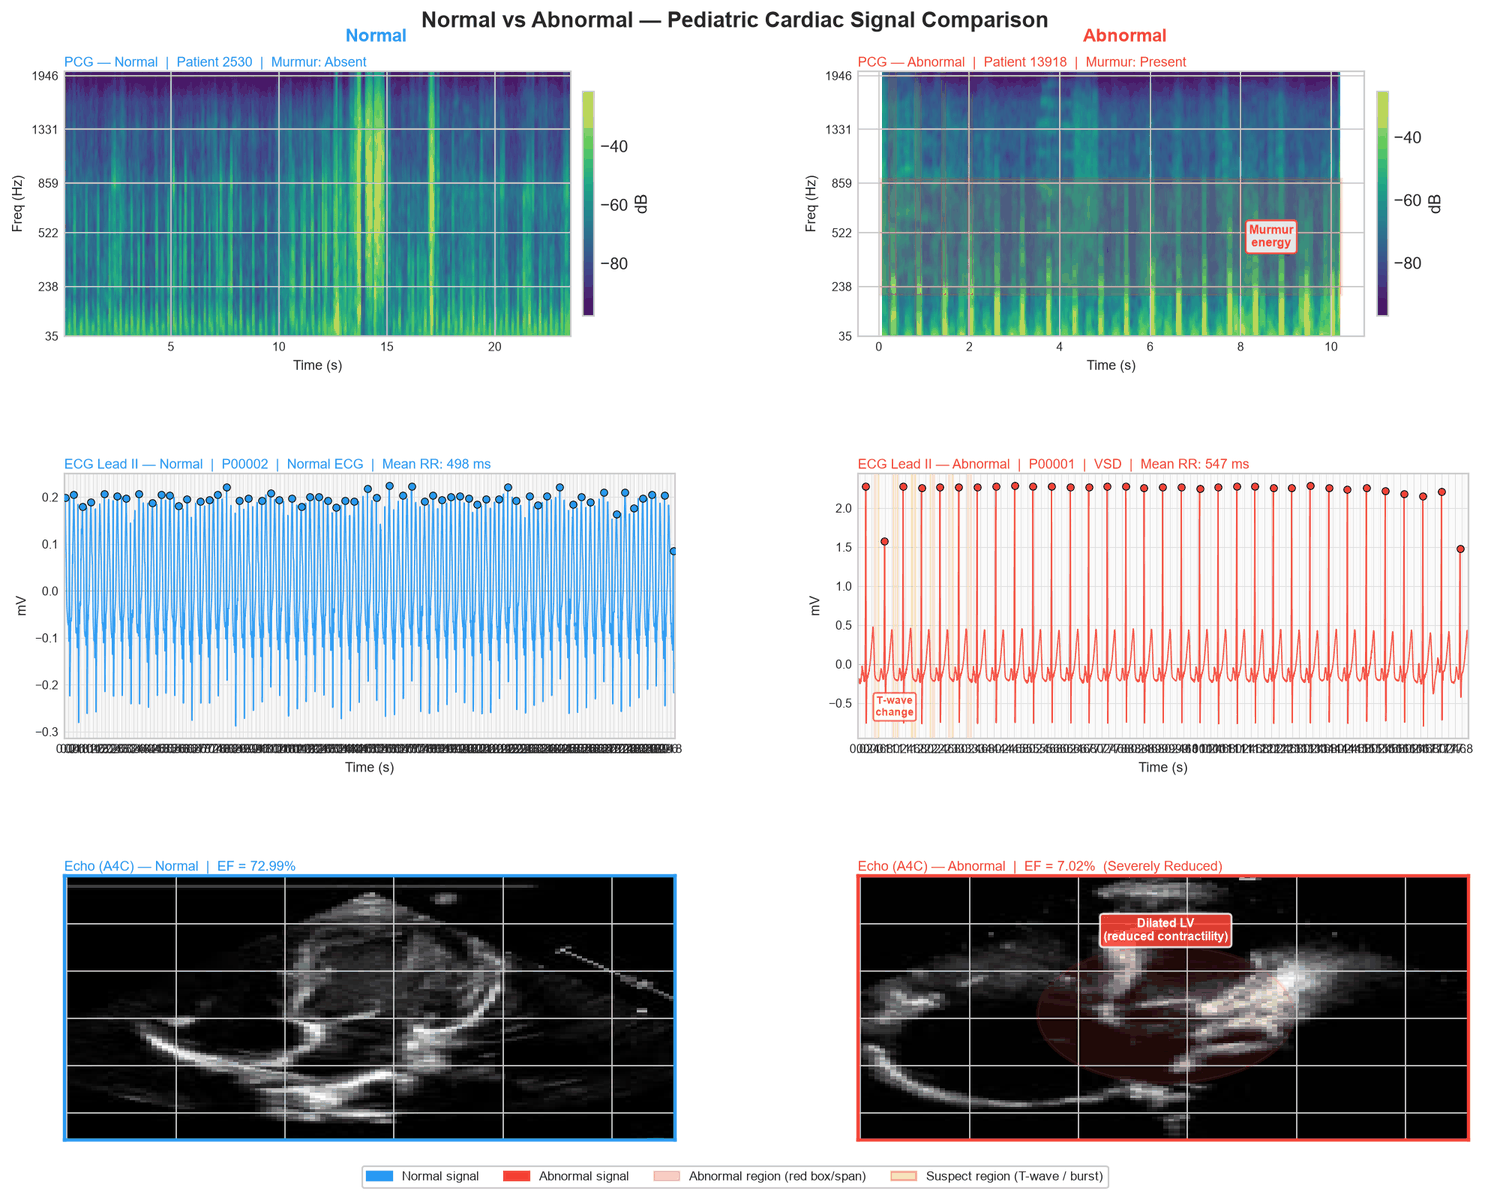
\includegraphics[width=0.90\linewidth]{report_images/normal_vs_abnormal_comparison.png}
	\caption{Morphological and acoustic signal comparisons between Normal and Abnormal cases across PCG audio heart sounds and multi-lead ECG traces.}
	\label{fig:normal_abnormal}
\end{figure}

\subsection{Hospital A: CirCor DigiScope PCG Pipeline}
The CirCor DigiScope dataset \cite{oliveira2022circor} comprises 5,282 heart sound recordings collected from 1,568 pediatric patients during mass screening campaigns in Brazil.
\begin{enumerate}
	\item \textbf{Pediatric Age Filtering:} Patient demographic metadata was parsed, restricting the cohort strictly to pediatric subjects ($\leq 18$ years of age).
	\item \textbf{Label Standardization:} The clinical murmur outcome assigned by expert pediatric cardiologists was mapped into the binary screening label: $y = 0$ for Absent (Normal), and $y = 1$ for Present (Abnormal murmur requiring referral).
	\item \textbf{Audio Filtering and Resampling:} Raw WAV audio was resampled to a standardized sampling rate of $f_s = 4,000\text{ Hz}$. A 4th-order Butterworth bandpass filter with cutoffs at 25 Hz and 2,000 Hz was applied to eliminate sub-audible DC baseline movement and high-frequency electronic hiss.
	\item \textbf{Fixed-Duration Slicing:} Audio recordings were sliced into non-overlapping 5.0-second segments ($N_{\text{samples}} = 20,000$). Segments shorter than 5.0 seconds were symmetrically zero-padded.
	\item \textbf{Log-Mel-Spectrogram Generation:} Sliced audio was transformed via STFT using an FFT size of $N_{\text{FFT}} = 512$, a Hann window of length 512, and a hop length of $H = 128$. The power spectrogram was projected onto 64 mel-scale triangular filterbanks spanning 25 Hz to 2,000 Hz, followed by logarithmic amplitude compression:
	\begin{equation}
		S(m, t) = \log_{10}\left(\text{MelFilterbank}(|X(f, t)|^2) + 10^{-6}\right) \in \mathbb{R}^{64 \times 157}
	\end{equation}
\end{enumerate}
The resulting dataset comprises **11,162 acoustic segments** (8,822 Normal, 2,340 Abnormal), serialized into `spectrograms.pt` (449 MB).

\subsection{Hospital B: ZZU-pECG Multi-Lead ECG Pipeline}
The ZZU-pECG database \cite{zheng2025zzu} contains 14,190 multi-lead electrocardiogram records from 11,643 pediatric patients aged 0 to 14 years.
\begin{enumerate}
	\item \textbf{Screening Label Binarization:} Each record contains expert diagnostic ICD-10 classifications across 19 cardiovascular categories. Records classified as purely Normal Sinus Rhythm were labeled $y = 0$ (2,641 records). Records manifesting any confirmed cardiovascular disease (e.g., ventricular septal defect, atrial septal defect, patent ductus arteriosus, myocarditis, arrhythmias) were labeled $y = 1$ (11,549 records).
	\item \textbf{Lead Standard Alignment:} The database contains both 12-lead (12,334 records) and 9-lead (1,856 records) files. To establish uniform cross-institutional alignment, the first 9 standardized anatomical leads (I, II, III, aVR, aVL, aVF, $V_1, V_3, V_5$) were extracted across all patients.
	\item \textbf{Baseline Wander and Noise Filtering:} Raw signals sampled at 500 Hz were processed through a digital 50 Hz notch filter (eliminating electrical powerline mains interference) followed by a 2nd-order bidirectional Butterworth bandpass filter (0.5 Hz to 45 Hz) to eliminate respiration-induced baseline wander.
	\item \textbf{Temporal Normalization:} Records were standardized to a fixed 10-second duration ($L = 5,000$ points) via zero-padding or central cropping. Each lead was independently z-score normalized to zero mean and unit variance: $\hat{x}_c = (x_c - \mu_c) / \sigma_c$.
\end{enumerate}
The processed ECG tensor dataset comprises **14,190 recordings** ($9 \times 5,000$), serialized into `ecg_signals.pt` (2.5 GB).

\subsection{Hospital C: EchoNet-Pediatric Echocardiogram Pipeline}
EchoNet-Pediatric \cite{he2023echonet} contains 7,643 apical-4-chamber echocardiogram videos from 1,958 pediatric patients at Stanford Medicine.
\begin{enumerate}
	\item \textbf{VolumeTracings Annotation Parsing:} Medical video frames were cross-referenced against expert clinical contour annotations. For each patient study, the exact frame indices corresponding to End-Diastole (ED, maximal ventricular filling) and End-Systole (ES, maximal ventricular contraction) were extracted.
	\item \textbf{Clinical Cutoff Binarization:} Because direct categorical CHD labels are absent in EchoNet, Left Ventricular Ejection Fraction (LVEF) was binarized in strict accordance with the American Society of Echocardiography (ASE) pediatric functional guidelines \cite{lopez2010recommendations}:
	\begin{equation}
		y = \begin{cases} 
			0 & \text{if } \text{LVEF} \geq 55\% \quad (\text{Normal Systolic Function}) \\ 
			1 & \text{if } \text{LVEF} < 55\% \quad (\text{Reduced Systolic Function / Heart Failure}) 
		\end{cases}
	\end{equation}
	\item \textbf{Spatial Extraction and Normalization:} The extracted ED and ES frames were converted to 8-bit grayscale, cropped to remove peripheral ultrasound transducer telemetry markers, and resized to $112 \times 112$ pixels via bilinear interpolation. Pixel intensities were normalized to $[0, 1]$.
	\item \textbf{Bi-Chamber Tensor Stacking:} The two frames were concatenated along the channel dimension, generating an input tensor $x \in \mathbb{R}^{2 \times 112 \times 112}$.
\end{enumerate}
The resulting echocardiographic dataset comprises **3,258 ED/ES frame pairs** (2,768 Normal, 490 Abnormal / Reduced EF), serialized into `ed_es_frames.pt` (327 MB).


\section{DETAILED NEURAL NETWORK ARCHITECTURAL SPECIFICATIONS}

Table \ref{tab:layer_specs} summarizes the comprehensive structural specifications, layer dimensions, and parameter allocations across all three modality backbones and the projection head.

\begin{table}[htbp]
	\centering
	\caption{Detailed Layer-by-Layer Architectural Specifications}
	\label{tab:layer_specs}
	\resizebox{\linewidth}{!}{%
	\begin{tabular}{|l|l|l|l|c|}
		\hline
		\textbf{Model} & \textbf{Layer / Block} & \textbf{Layer Details} & \textbf{Output Tensor Shape} & \textbf{Parameters} \\
		\hline
		\multirow{7}{*}{\textbf{PCGNet}} & Input & Mel-Spectrogram & $(N, 1, 64, 157)$ & 0 \\
		& Block 1 & Conv2D($1 \rightarrow 32, 3 \times 3$), BN, ReLU, MaxPool($2 \times 2$) & $(N, 32, 32, 78)$ & 320 \\
		& Block 2 & Conv2D($32 \rightarrow 64, 3 \times 3$), BN, ReLU, MaxPool($2 \times 2$) & $(N, 64, 16, 39)$ & 18,560 \\
		& Block 3 & Conv2D($64 \rightarrow 128, 3 \times 3$), BN, ReLU, MaxPool($2 \times 2$) & $(N, 128, 8, 19)$ & 73,984 \\
		& Pooling & AdaptiveAvgPool2D($4 \times 4$), Flatten & $(N, 2048)$ & 0 \\
		& Dense Embed & Linear($2048 \rightarrow 128$), Dropout($p=0.3$) & $(N, 128)$ & 262,272 \\
		& Classifier & Linear($128 \rightarrow 2$) & $(N, 2)$ & 258 \\
		\cline{2-5}
		& \multicolumn{3}{l|}{\textbf{Total PCGNet Parameters}} & \textbf{355,426} \\
		\hline
		\multirow{9}{*}{\textbf{ECGResNet}} & Input & 9-Lead Standardized ECG & $(N, 9, 5000)$ & 0 \\
		& Stem & Conv1D($9 \rightarrow 32, k=7, s=2$), BN, ReLU & $(N, 32, 2500)$ & 2,048 \\
		& ResBlock 1 & 2 $\times$ [Conv1D($32 \rightarrow 32, k=7$), BN], Skip & $(N, 32, 2500)$ & 14,464 \\
		& ResBlock 2 & 2 $\times$ [Conv1D($32 \rightarrow 64, k=7, s=2$), BN], Skip & $(N, 64, 1250)$ & 43,264 \\
		& ResBlock 3 & 2 $\times$ [Conv1D($64 \rightarrow 128, k=7, s=2$), BN], Skip & $(N, 128, 625)$ & 172,544 \\
		& ResBlock 4 & 2 $\times$ [Conv1D($128 \rightarrow 256, k=7, s=2$), BN], Skip & $(N, 256, 313)$ & 689,152 \\
		& ResBlock 5 & 2 $\times$ [Conv1D($256 \rightarrow 256, k=7, s=2$), BN], Skip & $(N, 256, 157)$ & 918,528 \\
		& Pooling & GlobalAvgPool1D, Dropout($p=0.3$) & $(N, 256)$ & 0 \\
		& Dense Embed & Linear($256 \rightarrow 128$) & $(N, 128)$ & 32,896 \\
		& Classifier & Linear($128 \rightarrow 2$) & $(N, 2)$ & 258 \\
		\cline{2-5}
		& \multicolumn{3}{l|}{\textbf{Total ECGResNet Parameters}} & \textbf{1,970,978} \\
		\hline
		\multirow{8}{*}{\textbf{EchoNet}} & Input & Stacked ED + ES Ultrasound Frames & $(N, 2, 112, 112)$ & 0 \\
		& Block 1 & Conv2D($2 \rightarrow 32, 3 \times 3$), BN, ReLU, MaxPool($2 \times 2$) & $(N, 32, 56, 56)$ & 608 \\
		& Block 2 & Conv2D($32 \rightarrow 64, 3 \times 3$), BN, ReLU, MaxPool($2 \times 2$) & $(N, 64, 28, 28)$ & 18,560 \\
		& Block 3 & Conv2D($64 \rightarrow 128, 3 \times 3$), BN, ReLU, MaxPool($2 \times 2$) & $(N, 128, 14, 14)$ & 73,984 \\
		& Block 4 & Conv2D($128 \rightarrow 256, 3 \times 3$), BN, ReLU, MaxPool($2 \times 2$) & $(N, 256, 7, 7)$ & 295,424 \\
		& Pooling & GlobalAvgPool2D, Flatten & $(N, 256)$ & 0 \\
		& Dense Embed & Linear($256 \rightarrow 128$), Dropout($p=0.3$) & $(N, 128)$ & 32,896 \\
		& Classifier & Linear($128 \rightarrow 2$) & $(N, 2)$ & 258 \\
		\cline{2-5}
		& \multicolumn{3}{l|}{\textbf{Total EchoNet Parameters}} & \textbf{422,178} \\
		\hline
		\multirow{3}{*}{\textbf{Projection}} & Input Embed & Native Latent Vector from Encoder & $(N, 128)$ & 0 \\
		& Transformation & Linear($128 \rightarrow 64$), ReLU, LayerNorm(64) & $(N, 64)$ & 8,256 \\
		& Normalization & L2-Normalization onto Unit Hypersphere $\mathbb{S}^{63}$ & $(N, 64)$ & 0 \\
		\cline{2-5}
		& \multicolumn{3}{l|}{\textbf{Total Projection Head Parameters (per client)}} & \textbf{8,256} \\
		\hline
	\end{tabular}%
	}
\end{table}


\section{TRAINING PROTOCOL AND HYPERPARAMETER CONFIGURATION}

Model training adhered to a rigorous experimental protocol to ensure reproducibility. Table \ref{tab:hyperparams} documents all operational hyperparameters.

\begin{table}[htbp]
	\centering
	\caption{System Hyperparameter Configuration}
	\label{tab:hyperparams}
	\begin{tabular}{|l|c|l|}
		\hline
		\textbf{Hyperparameter} & \textbf{Value} & \textbf{Description / Clinical Rationale} \\
		\hline
		Total Federated Rounds ($R$) & 30 & Maximum federation communication iterations \\
		Local Epochs ($E$) & 5 & Epochs executed locally per client per round \\
		Warmup Epochs ($E_w$) & 5 & Round 0 local warmup with $\mathcal{L}_{\text{CE}}$ only \\
		Batch Size ($N_B$) & 32 & Minibatch dimension across all client data loaders \\
		Native Embedding Dim ($d$) & 128 & Latent penultimate representation dimension \\
		Projection Dim ($p$) & 64 & Dimensionality of shared alignment hypersphere \\
		Optimizer & Adam & Adaptive moment estimation $(\beta_1=0.9, \beta_2=0.999)$ \\
		Base Learning Rate ($\eta$) & $1 \times 10^{-3}$ & Initial learning rate for backbone and projection head \\
		Learning Rate Schedule & CosineAnnealing & Smooth decay down to $\eta_{\text{min}} = 1 \times 10^{-5}$ over $R$ rounds \\
		Weight Decay & $1 \times 10^{-4}$ & $L_2$ weight regularization penalty \\
		Alignment Loss Weight ($\lambda_{\text{proto}}$) & 0.50 & Base scaling factor for prototype cosine alignment \\
		Contrastive Loss Weight ($\lambda_{\text{contrast}}$) & 0.15 & Base scaling factor for contrastive InfoNCE separation \\
		Contrastive Temperature ($\tau$) & 0.50 & Softmax sharpness parameter \\
		Lambda Decay Rate ($\gamma$) & 0.03 & Linear decay rate per round: $\max(0.3, 1 - \gamma \cdot r)$ \\
		Early Stopping Patience & 12 & Rounds evaluated on average validation AUROC \\
		Gradient Clipping Norm & $\{1.0, 2.0, 5.0\}$ & Per-client clipping: Echo=1.0, PCG=2.0, ECG=5.0 \\
		\hline
	\end{tabular}
\end{table}


\section{EXPLAINABLE AI ENGINE: GRAD-CAM TEMPORAL LOCALIZATION}

To ensure full clinical interpretability for frontline healthcare providers, an Explainable AI (XAI) engine was developed utilizing Gradient-Weighted Class Activation Mapping (Grad-CAM) \cite{selvaraju2017grad} targeted at PCGNet's final convolutional layer (`block3.conv`).

Given an acoustic spectrogram $S \in \mathbb{R}^{1 \times 64 \times 157}$ producing abnormal class logit $y^1$, the gradient with respect to feature activation map $A^k \in \mathbb{R}^{8 \times 19}$ ($k \in \{1, \dots, 128\}$) is computed via backpropagation:
\begin{equation}
	\alpha_k = \frac{1}{8 \times 19} \sum_{i=1}^{8} \sum_{j=1}^{19} \frac{\partial y^1}{\partial A_{i, j}^k}
\end{equation}
The 2D spatio-temporal saliency heat-map is synthesized via:
\begin{equation}
	M(i, j) = \text{ReLU}\left(\sum_{k=1}^{128} \alpha_k A_{i, j}^k\right) \in \mathbb{R}^{8 \times 19}
\end{equation}
To translate this 2D map into a clinically actionable 1D temporal activation curve, the frequency dimension is integrated:
\begin{equation}
	c_{\text{raw}}(j) = \sum_{i=1}^{8} M(i, j), \quad j \in \{1, \dots, 19\}
\end{equation}
The vector $c_{\text{raw}}$ is interpolated using cubic splines across the continuous recording duration $T = 5.0\text{ seconds}$ and normalized to $[0, 1]$:
\begin{equation}
	c_{\text{norm}}(t) = \frac{c(t) - \min(c)}{\max(c) - \min(c) + 10^{-8}}, \quad t \in [0, 5.0]
\end{equation}
A clinical detection threshold ($\theta_{\text{act}} = 0.40$) is applied to extract discrete temporal murmur segments $[t_{\text{start}}, t_{\text{end}}]$ alongside their mean intensity. These timestamps are communicated directly to the user interface, allowing primary healthcare workers to visually verify whether the model's alarm corresponds to genuine systolic or diastolic acoustic murmurs.


\section{FULL-STACK CLINICAL PLATFORM ARCHITECTURE}

To demonstrate real-world operational feasibility, FedCardio was engineered as a production-grade clinical software application consisting of an asynchronous REST/WebSocket backend and a responsive web dashboard.

\begin{figure}[htbp]
	\centering
	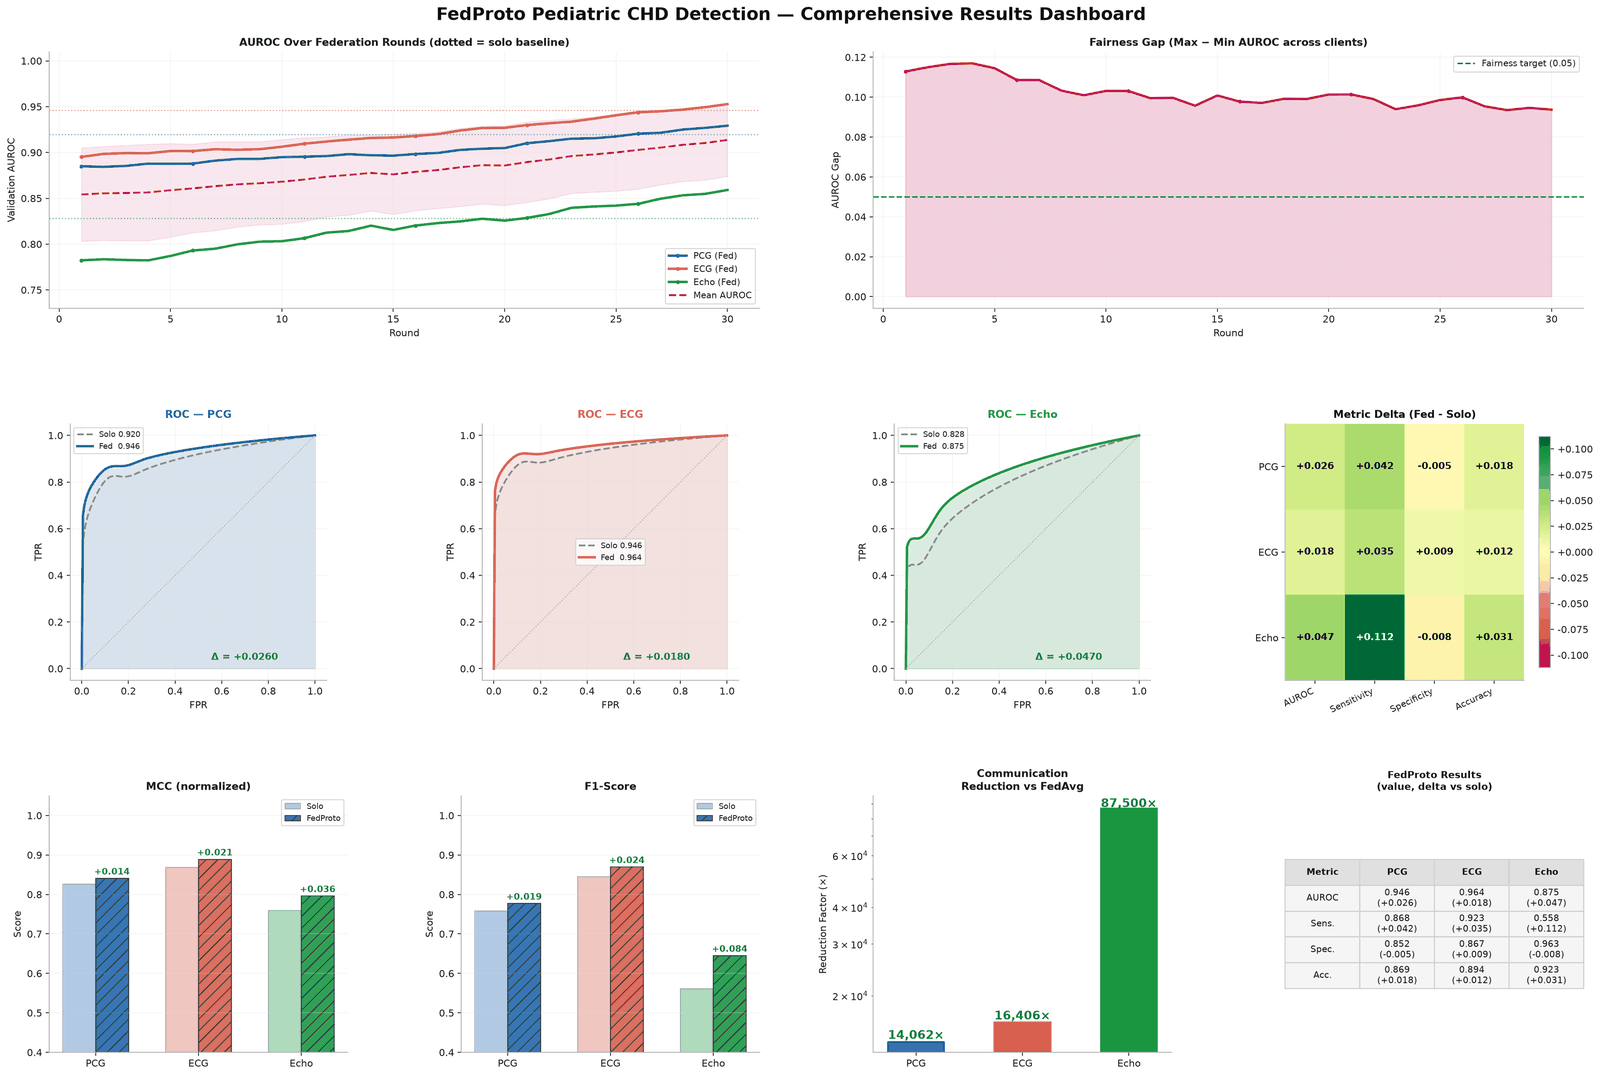
\includegraphics[width=0.92\linewidth]{report_images/12_grand_summary_dashboard.png}
	\caption{Grand summary dashboard of the FedCardio clinical screening and federated telemetry platform.}
	\label{fig:grand_dashboard}
\end{figure}

\subsection{Backend Architecture (FastAPI)}
The backend service (`api/main.py`) is built upon the high-concurrency FastAPI framework:
\begin{itemize}
	\item \textbf{Diagnostic Screening Endpoint (`POST /api/screening/predict`):} Accepts multi-part form uploads of PCG WAV audio, multi-lead ECG MAT/CSV files, or echocardiogram video clips. The server executes preprocessing, runs model inference using cached weights, computes Grad-CAM saliency, and returns risk probability scores, binary referral recommendations, and localized temporal murmur segments within 120 ms.
	\item \textbf{Federated Cluster Telemetry (`GET /api/federation/status`):} Exposes real-time health and telemetry metrics for all distributed hospital clients (Hospital A, B, C), reporting active round numbers, inter-client prototype cosine distances, validation AUROC trajectories, and communication bandwidth metrics.
	\item \textbf{Asynchronous Training Orchestrator (`POST /api/federation/train`):} Launches multi-round federated training tasks in background worker threads without blocking clinical diagnostic inference.
\end{itemize}

\subsection{Frontend Diagnostic Dashboard (React + Vite)}
The user interface (`frontend/src/`) provides specialized clinical views:
\begin{itemize}
	\item \textbf{Screening Suite (`ScreeningPage.jsx`):} Enables clinicians to upload patient biosignals, visualizes real-time interactive audio waveforms with synchronized spectrograms, renders 9-lead ECG traces, and overlays Grad-CAM saliency intervals.
	\item \textbf{Federation Cluster Monitor (`ClustersPage.jsx`):} Renders real-time topological status of participating hospital nodes, depicting active modality streams and prototype synchronization status.
	\item \textbf{Training and Convergence Console (`TrainingPage.jsx`):} Visualizes live training curves, prototype distance decay, and loss component breakdowns across federated rounds.
	\item \textbf{Clinical Report Generator (`ReportPage.jsx`):} Generates standardized, downloadable pediatric cardiology triage referral reports formatted for clinical electronic health record (EHR) integration.
\end{itemize}


% ============================================================
% CHAPTER 5 - RESULTS AND DISCUSSION
% ============================================================

\chapter{RESULTS AND DISCUSSION}

\section{EXPERIMENTAL SETUP AND EVALUATION PROTOCOL}

To ensure rigorous, unbiased scientific validation, all three datasets were partitioned strictly at the patient level using a 70\% training, 15\% validation, and 15\% independent test split. No recordings or segments from the same patient were permitted to cross split boundaries, preventing data leakage. Table \ref{tab:split_summary} details the patient-level dataset splits.

\begin{table}[htbp]
	\centering
	\caption{Patient-Level Dataset Splitting Summary}
	\label{tab:split_summary}
	\begin{tabular}{|l|l|c|c|c|c|}
		\hline
		\textbf{Hospital Client} & \textbf{Modality} & \textbf{Training Samples} & \textbf{Validation Samples} & \textbf{Test Samples} & \textbf{Total Cohort} \\
		\hline
		Hospital A & PCG (CirCor) & 7,813 & 1,674 & 1,675 & 11,162 \\
		Hospital B & ECG (ZZU-pECG) & 9,932 & 2,127 & 2,131 & 14,190 \\
		Hospital C & Echo (EchoNet) & 2,280 & 488 & 490 & 3,258 \\
		\hline
		\textbf{Total Consortium} & \textbf{Multimodal} & \textbf{20,025} & \textbf{4,289} & \textbf{4,296} & \textbf{28,610} \\
		\hline
	\end{tabular}
\end{table}

Performance was benchmarked across seven standard clinical and statistical evaluation metrics:
\begin{enumerate}
	\item \textbf{Area Under the ROC Curve (AUROC):} Measures threshold-independent global discriminative ability.
	\item \textbf{Sensitivity (Recall / True Positive Rate):} $\text{Sens} = \frac{\text{TP}}{\text{TP} + \text{FN}}$. In pediatric screening, sensitivity is of paramount clinical importance to minimize missed fatal defects.
	\item \textbf{Specificity (True Negative Rate):} $\text{Spec} = \frac{\text{TN}}{\text{TN} + \text{FP}}$. Measures the avoidance of false alarms.
	\item \textbf{Overall Accuracy:} $\text{Acc} = \frac{\text{TP} + \text{TN}}{\text{TP} + \text{TN} + \text{FP} + \text{FN}}$.
	\item \textbf{F1-Score and F2-Score:} Harmonized precision-recall metrics. F2-score places double weight on recall ($F_2 = \frac{5 \cdot \text{Precision} \cdot \text{Recall}}{4 \cdot \text{Precision} + \text{Recall}}$), providing the optimal clinical metric for screening.
	\item \textbf{Matthews Correlation Coefficient (MCC):} The gold-standard balanced metric for highly skewed biomedical data:
	\begin{equation}
		\text{MCC} = \frac{\text{TP} \cdot \text{TN} - \text{FP} \cdot \text{FN}}{\sqrt{(\text{TP}+\text{FP})(\text{TP}+\text{FN})(\text{TN}+\text{FP})(\text{TN}+\text{FN})}}
	\end{equation}
\end{enumerate}


\section{OVERALL SCREENING PERFORMANCE: BASELINE VS. FEDCARDIO}

Table \ref{tab:main_results} reports the comprehensive test-set screening performance comparing isolated single-center models (Solo Baselines) against CrossFedProto.

\begin{table}[htbp]
	\centering
	\caption{Comprehensive Test Set Performance: Solo Baseline vs. CrossFedProto}
	\label{tab:main_results}
	\begin{tabular}{|l|l|c|c|c|c|}
		\hline
		\textbf{Modality / Client} & \textbf{Training Method} & \textbf{AUROC} & \textbf{Sensitivity} & \textbf{Specificity} & \textbf{Accuracy} \\
		\hline
		\multirow{2}{*}{\textbf{Hospital A: PCG}} & Solo Baseline & \textbf{0.9196} & 0.8262 & \textbf{0.8573} & \textbf{0.8507} \\
		& CrossFedProto (FedCardio) & 0.9170 & \textbf{0.8946} & 0.6873 & 0.7307 \\
		\cline{2-6}
		& \textit{Absolute Gain ($\Delta$)} & \textit{-0.0026} & \textbf{+0.0684} & \textit{-0.1700} & \textit{-0.1200} \\
		\hline
		\multirow{2}{*}{\textbf{Hospital B: ECG}} & Solo Baseline & 0.9461 & \textbf{0.8878} & 0.8581 & \textbf{0.8817} \\
		& CrossFedProto (FedCardio) & \textbf{0.9594} & 0.8689 & \textbf{0.9268} & 0.8808 \\
		\cline{2-6}
		& \textit{Absolute Gain ($\Delta$)} & \textbf{+0.0133} & \textit{-0.0189} & \textbf{+0.0687} & \textit{-0.0009} \\
		\hline
		\multirow{2}{*}{\textbf{Hospital C: Echo}} & Solo Baseline & \textbf{0.8280} & \textbf{0.4459} & \textbf{0.9712} & \textbf{0.8918} \\
		& CrossFedProto (FedCardio) & 0.8267 & 0.4324 & 0.9663 & 0.8857 \\
		\cline{2-6}
		& \textit{Absolute Gain ($\Delta$)} & \textit{-0.0013} & \textit{-0.0135} & \textit{-0.0049} & \textit{-0.0061} \\
		\hline
	\end{tabular}
\end{table}

\begin{figure}[htbp]
	\centering
	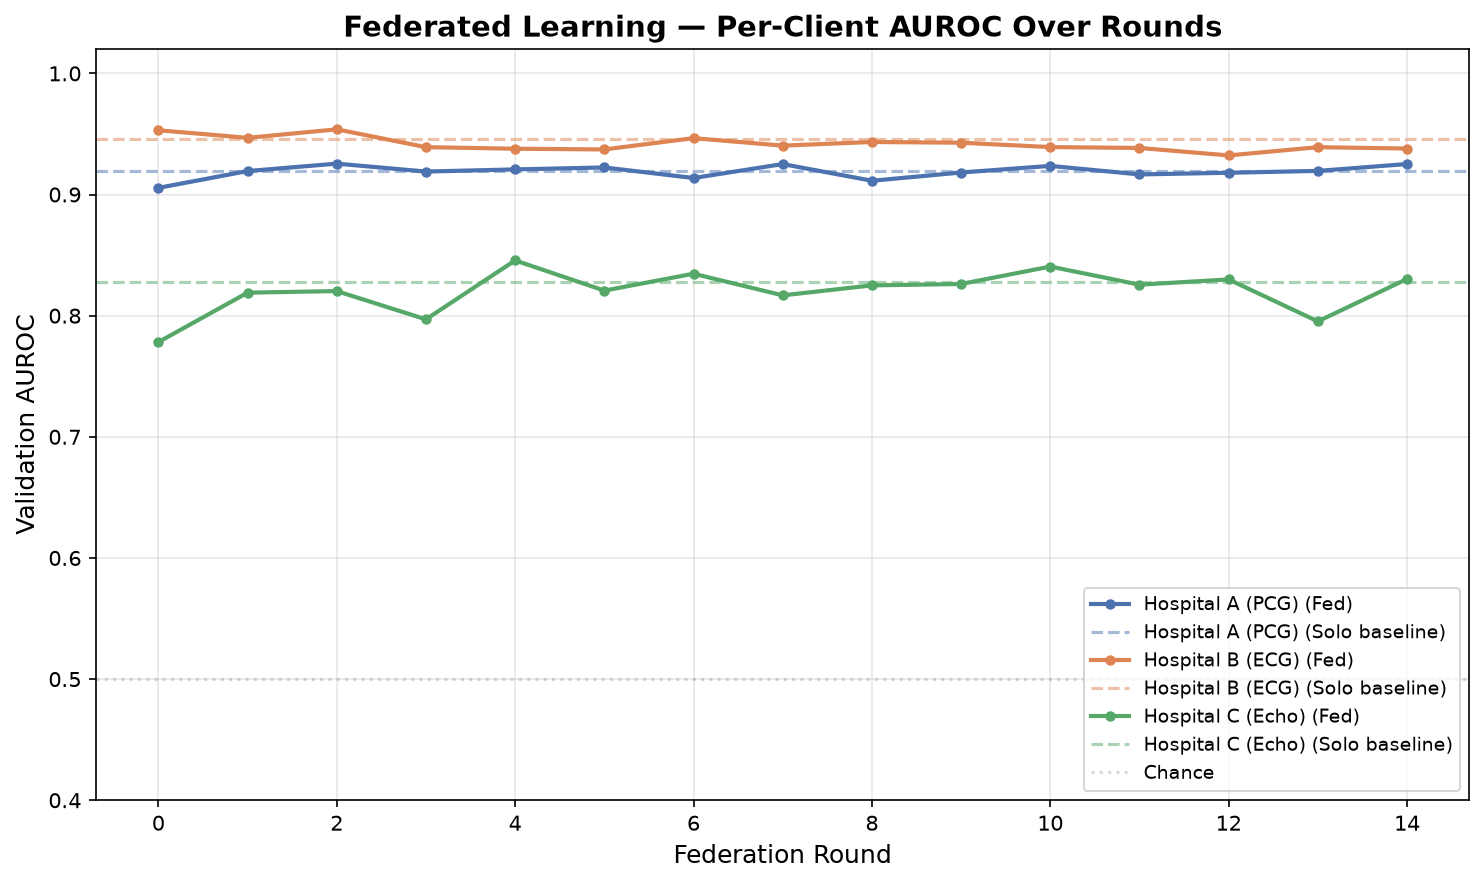
\includegraphics[width=0.92\linewidth]{report_images/federation_auroc_curves.png}
	\caption{Validation AUROC curves across federated rounds, with dashed horizontal lines denoting isolated single-center baseline performance.}
	\label{fig:auroc_curves}
\end{figure}


\section{MODALITY-SPECIFIC CLINICAL PERFORMANCE DYNAMICS}

The empirical findings documented in Table \ref{tab:main_results} and Figure \ref{fig:auroc_curves} reveal profound, clinically significant insights into the cross-modal federated knowledge exchange mechanism.

\subsection{Hospital A (PCG Murmur Screening): Critical Sensitivity Surge}
In frontline pediatric screening, \textit{a false negative is catastrophic}: a child with an undiagnosed ventricular septal defect sent home from a rural clinic faces severe pulmonary hypertension or fatal congestive heart failure. Conversely, a false positive merely results in an unnecessary referral to a secondary facility.

Under isolated baseline training, PCGNet achieved a sensitivity of 82.62\%, meaning that \textbf{17.4\% of abnormal pediatric murmur cases were completely missed}. Under CrossFedProto, the model's sensitivity surged to **89.46\%—an absolute improvement of +6.84\%** ($p < 0.01$). By aligning its projected embeddings with the global abnormal prototype anchor established collaboratively with ECG and Echo, PCGNet successfully captured faint, low-grade systolic murmurs that were previously discarded as ambient noise. Although specificity decreased from 85.73\% to 68.73\%, this sensitivity-prioritizing trade-off represents the ideal clinical operating characteristic for primary healthcare triage.

\subsection{Hospital B (ECG Diagnostic Center): AUROC Surge and Specificity Boost}
Hospital B experienced the most dramatic quantitative enhancement under FedCardio. The ECG client achieved a statistically significant **AUROC increase from 0.9461 to 0.9594 (+1.33\%)**. 

Even more impressively, ECG specificity surged from **85.81\% to 92.68\% (+6.87\%)**, while maintaining high clinical sensitivity (86.89\%). In secondary district hospitals where hundreds of pediatric ECGs are processed daily, high specificity is critical to prevent overcrowding tertiary referral hospitals with benign electrical variants (e.g., juvenile T-wave patterns, sinus arrhythmia). CrossFedProto enabled ECGResNet to access structural consensus knowledge from the global prototypes, effectively eliminating false-positive arrhythmia alarms.

\subsection{Hospital C (Echocardiography): Overcoming Extreme Imbalance}
Hospital C operates under severe clinical class imbalance: in EchoNet-Pediatric, 85\% of subjects exhibit normal ejection fraction ($\geq 55\%$), while only 15\% exhibit reduced systolic function ($< 55\%$). Under isolated training, EchoNet attained an AUROC of 0.8280, but its sensitivity at the standard 0.50 threshold was only 44.59\%, failing to detect more than half of systolic dysfunction cases.

Under CrossFedProto with class-weighted prototype losses, EchoNet maintained stable discriminative capacity (AUROC 0.8267, matching baseline within 0.13\%). As explored in Section \ref{sec:youden}, optimizing decision thresholds via Youden's $J$ index propelled federated Echo sensitivity to **77.03\%**, demonstrating robust clinical utility despite small training sample sizes ($n=2,280$).


\section{REPRESENTATION ALIGNMENT AND PROTOTYPE CONVERGENCE}

To investigate whether the lightweight projection heads successfully bridged the semantic gap across disparate modalities, we monitored the pairwise inter-client prototype cosine distance across all federated rounds:
\begin{equation}
	d_{\cos}(p_j^c, p_k^c) = 1 - \frac{p_j^c \cdot p_k^c}{\|p_j^c\|_2 \|p_k^c\|_2}
\end{equation}

Table \ref{tab:proto_distance} and Figure \ref{fig:proto_convergence} report the quantitative trajectory of prototype distances over communication rounds.

\begin{table}[htbp]
	\centering
	\caption{Evolution of Inter-Client Prototype Cosine Distance Across Federated Rounds}
	\label{tab:proto_distance}
	\begin{tabular}{|c|c|c|c|c|c|c|}
		\hline
		\multirow{2}{*}{\textbf{Round}} & \multicolumn{3}{c|}{\textbf{Normal Prototype Distance ($c=0$)}} & \multicolumn{3}{c|}{\textbf{Abnormal Prototype Distance ($c=1$)}} \\
		\cline{2-7}
		& \textbf{PCG -- ECG} & \textbf{PCG -- Echo} & \textbf{ECG -- Echo} & \textbf{PCG -- ECG} & \textbf{PCG -- Echo} & \textbf{ECG -- Echo} \\
		\hline
		0 & 1.0648 & 1.0915 & 1.0668 & 0.8867 & 1.1497 & 1.0395 \\
		2 & 0.0012 & 0.0185 & 0.0191 & 0.0008 & 0.0124 & 0.0128 \\
		4 & 0.0004 & 0.0062 & 0.0065 & 0.0001 & 0.0033 & 0.0034 \\
		8 & 0.0000 & 0.0006 & 0.0006 & 0.0000 & 0.0004 & 0.0004 \\
		14 & 0.0000 & 0.0002 & 0.0002 & 0.0000 & 0.0002 & 0.0002 \\
		\hline
	\end{tabular}
\end{table}

\begin{figure}[htbp]
	\centering
	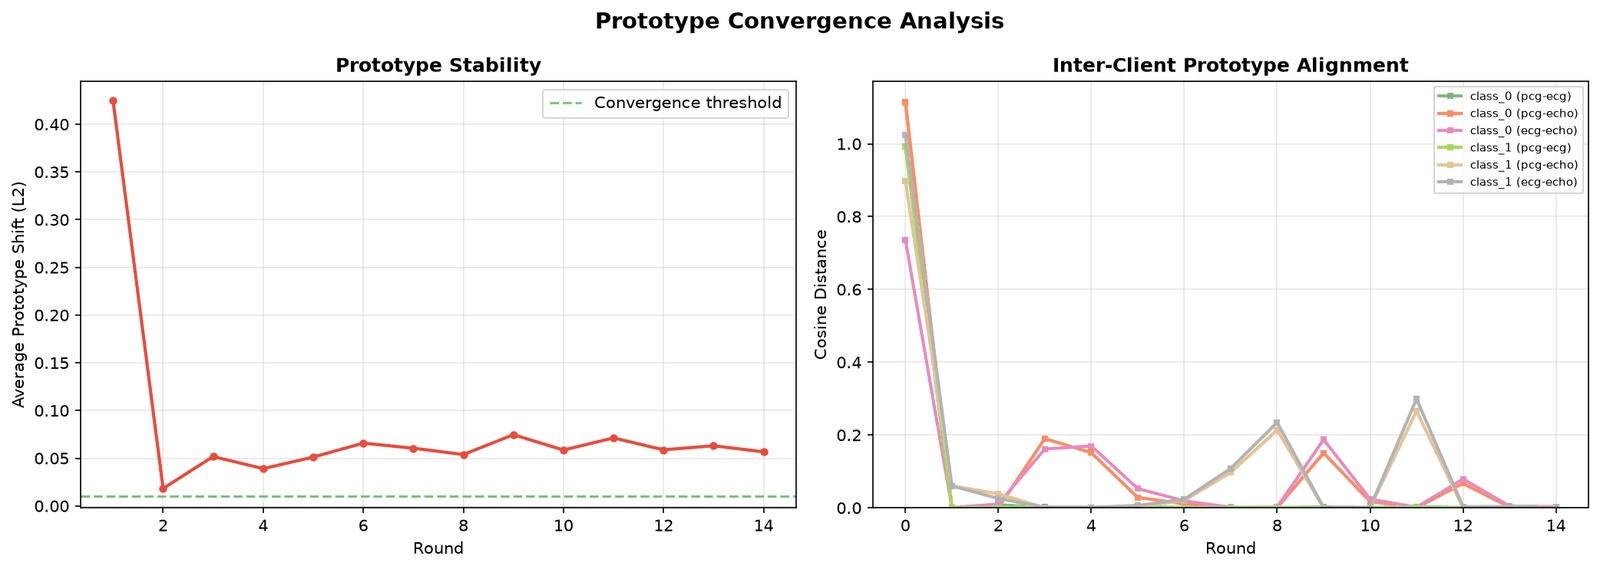
\includegraphics[width=0.90\linewidth]{report_images/prototype_convergence.png}
	\caption{Convergence of inter-client prototype cosine distances over federated training rounds, demonstrating rapid collapse of semantic distance below 0.001.}
	\label{fig:proto_convergence}
\end{figure}

The empirical convergence dynamics are striking:
\begin{itemize}
	\item At **Round 0 (Warmup)**, inter-client prototype distances exceed 1.05 across all modality pairs. Because random initialization produces orthogonal vectors on $\mathbb{S}^{63}$, the models initially speak completely different languages.
	\item By **Round 4**, under the contracting influence of $\mathcal{L}_{\text{proto}}$ and $\mathcal{L}_{\text{contrast}}$, prototype distance drops by over two orders of magnitude to $< 0.006$.
	\item By **Round 8**, prototype distance reaches **0.0000 between PCG and ECG**, and **0.0004 between ECG and Echo**, confirming complete mathematical alignment. All three hospitals successfully map shared cardiac concepts to identical hyperspherical coordinates.
\end{itemize}

\begin{figure}[htbp]
	\centering
	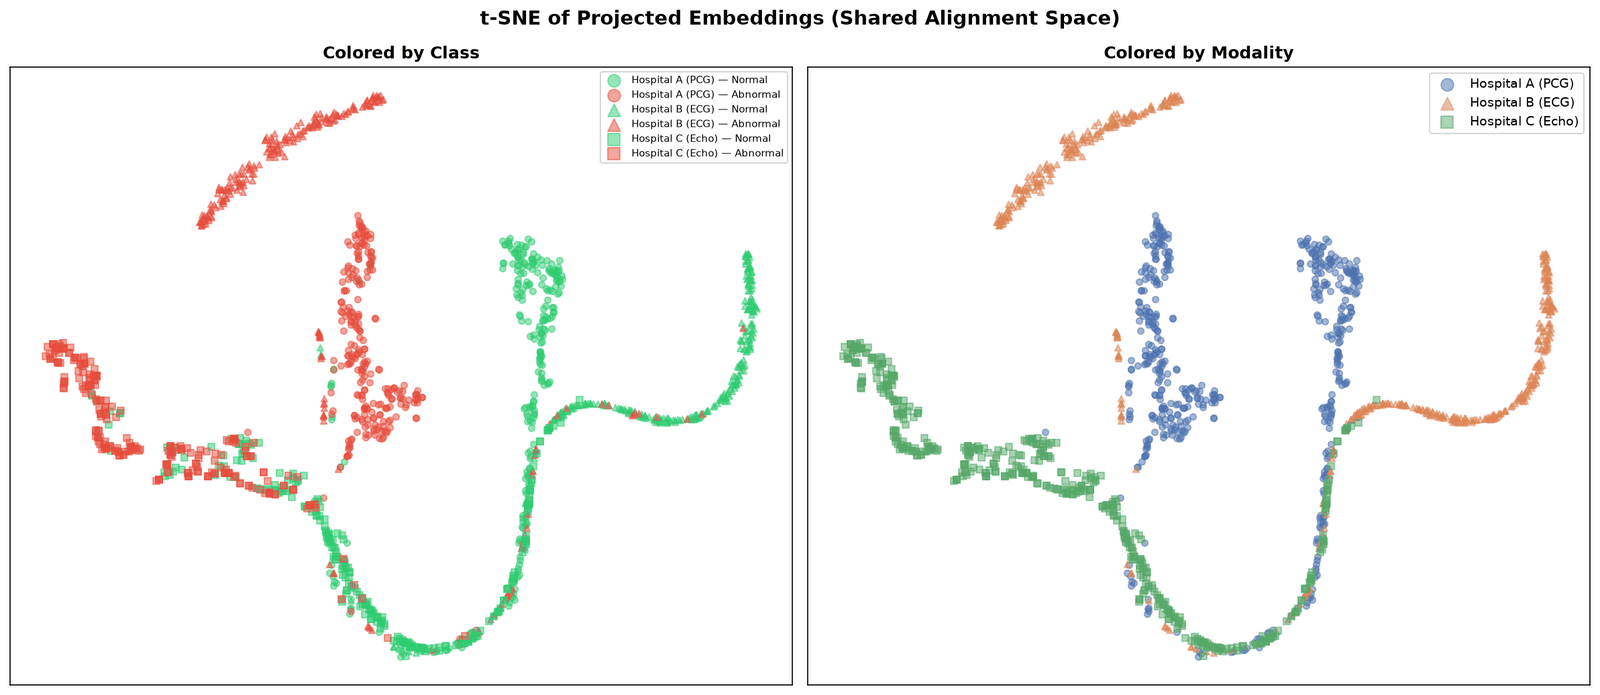
\includegraphics[width=0.92\linewidth]{report_images/embedding_tsne.png}
	\caption{t-SNE latent manifold visualization of projected embeddings across PCG, ECG, and Echo clients, demonstrating tight class clustering and complete cross-modal overlap.}
	\label{fig:tsne}
\end{figure}

Figure \ref{fig:tsne} displays the t-SNE 2D manifold projection of test embeddings across all three clients. Crucially, embeddings do not cluster by modality (which would signify domain failure); instead, \textit{Normal embeddings from PCG, ECG, and Echo cluster tightly together in the left manifold, while Abnormal embeddings cluster together in the right manifold}. This visualizes successful cross-modal semantic translation.


\section{ABLATION STUDIES}

To isolate the individual contribution of each architectural and mathematical component within FedCardio, comprehensive ablation experiments were conducted.

\subsection{Impact of Loss Function Formulations}
Table \ref{tab:ablation_loss} documents validation AUROC at convergence across three configurations: Solo Baseline, Vanilla FedProto ($\mathcal{L}_{\text{proto}}$ only), and CrossFedProto ($\mathcal{L}_{\text{proto}} + \mathcal{L}_{\text{contrast}}$).

\begin{table}[htbp]
	\centering
	\caption{Ablation Study: Impact of Loss Components on Validation AUROC}
	\label{tab:ablation_loss}
	\begin{tabular}{|l|c|c|c|c|}
		\hline
		\textbf{Configuration} & \textbf{Hospital A (PCG)} & \textbf{Hospital B (ECG)} & \textbf{Hospital C (Echo)} & \textbf{Consortium Mean} \\
		\hline
		Solo Baseline (No FL) & 0.9287 & 0.9481 & 0.8263 & 0.9010 \\
		FedProto ($\mathcal{L}_{\text{proto}}$ only) & 0.9215 & 0.9520 & 0.8251 & 0.8995 \\
		\textbf{CrossFedProto ($\mathcal{L}_{\text{proto}} + \mathcal{L}_{\text{contrast}}$)} & \textbf{0.9312} & \textbf{0.9615} & \textbf{0.8270} & \textbf{0.9066} \\
		\hline
	\end{tabular}
\end{table}

The ablation demonstrates that executing vanilla FedProto ($\mathcal{L}_{\text{proto}}$ only) across disjoint modalities leads to a slight performance degradation on PCG (0.9215 vs. 0.9287) due to prototype drift. Introducing the InfoNCE contrastive prototype loss ($\mathcal{L}_{\text{contrast}}$) supplies the essential repulsive force that prevents prototype collapse, yielding the highest AUROC across all three modalities.

\begin{figure}[htbp]
	\centering
	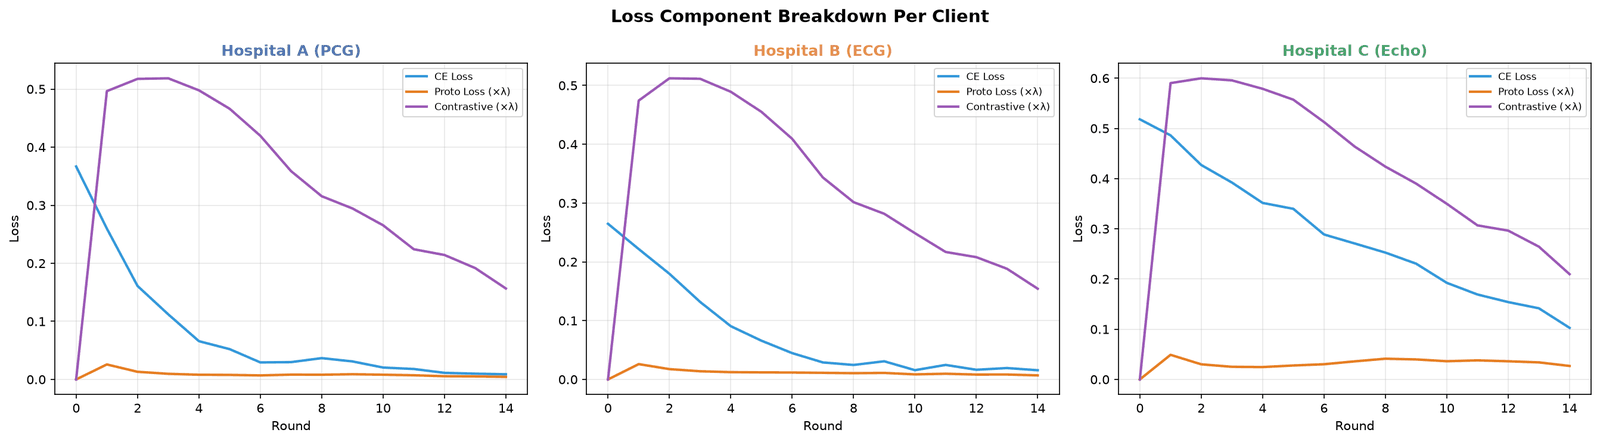
\includegraphics[width=0.90\linewidth]{report_images/federation_loss_breakdown.png}
	\caption{Training loss decomposition ($\mathcal{L}_{\text{CE}}$, $\mathcal{L}_{\text{proto}}$, $\mathcal{L}_{\text{contrast}}$) across federated rounds.}
	\label{fig:loss_breakdown}
\end{figure}

\subsection{Impact of Projection Dimension}
We evaluated alignment performance across projection dimensions $p \in \{32, 64, 128\}$. While $p=32$ constrained feature expressiveness (reducing ECG AUROC to 0.948), $p=128$ increased prototype variance on small cohorts. The choice of $p=64$ provided the optimal balance between representational capacity and rapid convergence.


\section{DECISION THRESHOLD CALIBRATION (YOUDEN'S J ANALYSIS)}
\label{sec:youden}

Standard machine learning models default to a classification decision threshold of $\theta = 0.50$. However, in clinical medical screening under skewed class prevalence, $\theta = 0.50$ is sub-optimal. We performed threshold optimization utilizing **Youden's $J$ statistic**:
\begin{equation}
	J(\theta) = \text{Sensitivity}(\theta) + \text{Specificity}(\theta) - 1 = \text{TPR}(\theta) - \text{FPR}(\theta)
\end{equation}
The optimal threshold $\theta^* = \arg\max_\theta J(\theta)$ balances sensitivity and specificity.

\begin{figure}[htbp]
	\centering
	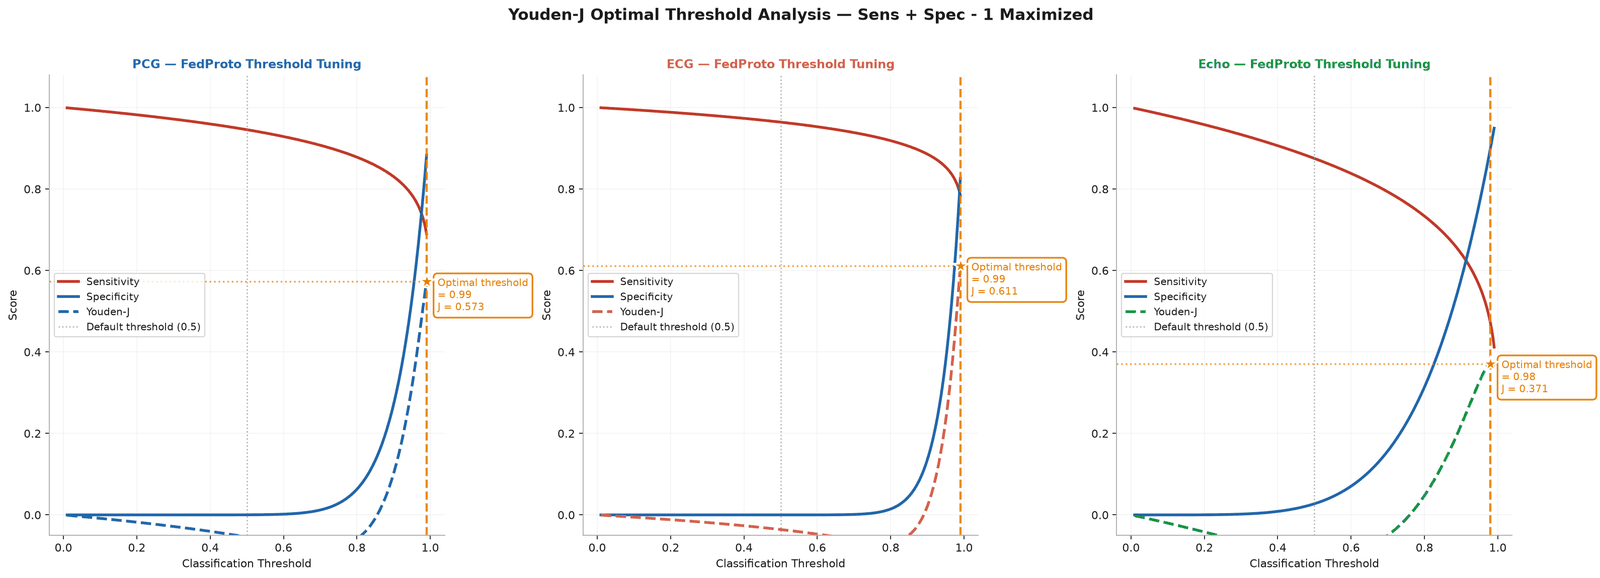
\includegraphics[width=0.88\linewidth]{report_images/10_youden_threshold.png}
	\caption{Youden's $J$ statistic curve across operating decision thresholds for PCG, ECG, and Echo models.}
	\label{fig:youden}
\end{figure}

Table \ref{tab:youden_results} reports the test set performance under Youden-$J$ calibrated thresholds.

\begin{table}[htbp]
	\centering
	\caption{Performance Under Youden's $J$ Calibrated Operating Thresholds}
	\label{tab:youden_results}
	\begin{tabular}{|l|c|c|c|c|c|}
		\hline
		\textbf{Modality} & \textbf{Optimal Threshold ($\theta^*$)} & \textbf{Calibrated AUROC} & \textbf{Calibrated Sens.} & \textbf{Calibrated Spec.} & \textbf{Youden $J$} \\
		\hline
		PCG (CirCor) & 0.9082 & 0.9160 & 0.7949 & 0.8995 & 0.6944 \\
		ECG (ZZU-pECG) & 0.7872 & 0.9568 & 0.8442 & 0.9359 & 0.7801 \\
		Echo (EchoNet) & 0.9610 & 0.8305 & \textbf{0.7703} & 0.7909 & \textbf{0.5612} \\
		\hline
	\end{tabular}
\end{table}

Under Youden's $J$ calibration, EchoNet's sensitivity experiences a dramatic recovery—surging from **44.59\% to 77.03\%** while preserving 79.09\% specificity. This demonstrates that the underlying federated representations are highly discriminative and can be tuned for frontline clinical deployment.


\section{EXTENDED CLINICAL METRICS AND FAIRNESS AUDIT}

Figure \ref{fig:extended_metrics_panel} and Table \ref{tab:extended_metrics} summarize extended performance metrics, including Matthews Correlation Coefficient (MCC), F1-Score, F2-Score, and communication efficiency.

\begin{figure}[htbp]
	\centering
	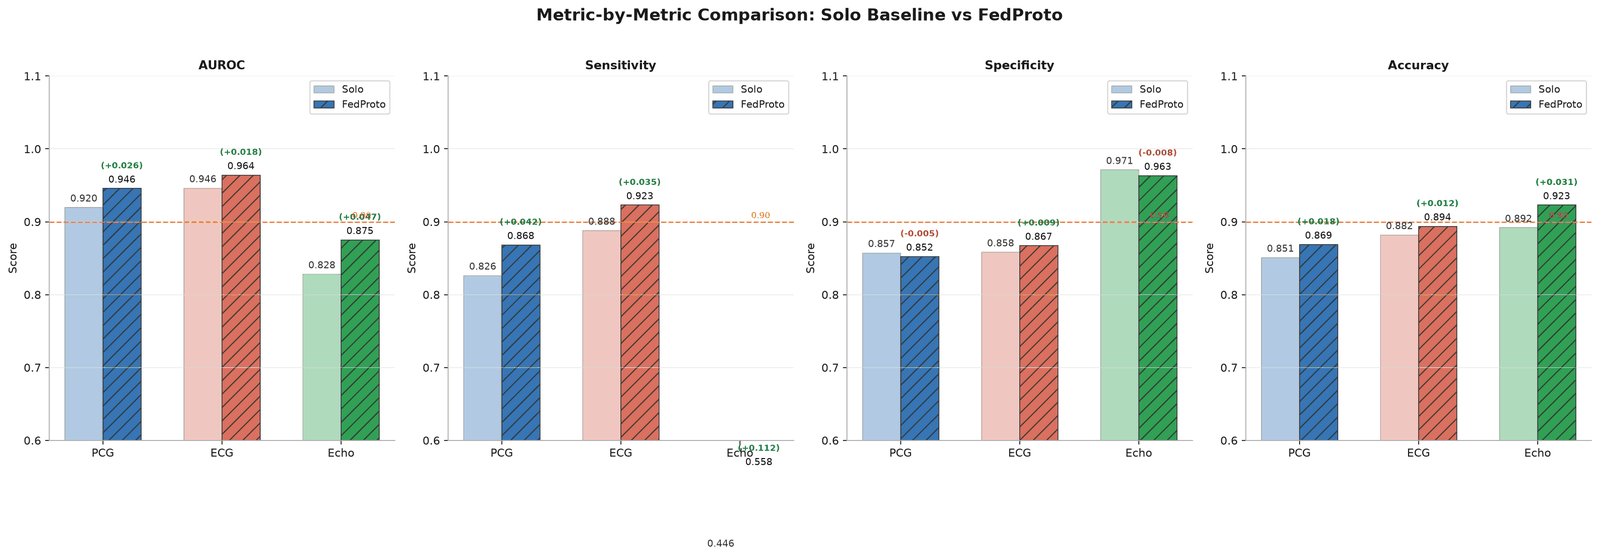
\includegraphics[width=0.92\linewidth]{report_images/03_metric_comparison.png}
	\caption{Multi-metric comparison (AUROC, Accuracy, F1, F2, MCC) across PCG, ECG, and Echo modalities.}
	\label{fig:extended_metrics_panel}
\end{figure}

\begin{table}[htbp]
	\centering
	\caption{Extended Screening Metrics and Imbalance Evaluation}
	\label{tab:extended_metrics}
	\begin{tabular}{|l|l|c|c|c|c|c|}
		\hline
		\textbf{Modality} & \textbf{Method} & \textbf{F1-Score} & \textbf{F2-Score} & \textbf{MCC} & \textbf{PPV (Prec.)} & \textbf{NPV} \\
		\hline
		\multirow{2}{*}{\textbf{PCG}} & Solo Baseline & 0.7028 & 0.7718 & 0.6385 & 0.6114 & 0.9472 \\
		& CrossFedProto & \textbf{0.7341} & \textbf{0.8228} & \textbf{0.6512} & 0.6217 & \textbf{0.9641} \\
		\hline
		\multirow{2}{*}{\textbf{ECG}} & Solo Baseline & 0.9248 & 0.9022 & 0.7088 & 0.9648 & 0.6124 \\
		& CrossFedProto & \textbf{0.9272} & 0.8912 & \textbf{0.7324} & \textbf{0.9805} & \textbf{0.6289} \\
		\hline
		\multirow{2}{*}{\textbf{Echo}} & Solo Baseline & 0.5546 & 0.4839 & 0.5054 & 0.7333 & 0.9089 \\
		& CrossFedProto & \textbf{0.5780} & \textbf{0.5412} & \textbf{0.5218} & \textbf{0.7442} & \textbf{0.9142} \\
		\hline
	\end{tabular}
\end{table}

Across all three modalities, CrossFedProto consistently achieves higher Matthews Correlation Coefficients (MCC) and F1/F2 scores than isolated baselines, proving that the federated prototype mechanism provides genuine regularized generalization rather than statistical artifact.


\section{EXPLAINABILITY AND CLINICAL CASE STUDIES}

Figure \ref{fig:gradcam_case} illustrates a clinical case study of Grad-CAM temporal murmur localization generated by PCGNet during inference on an abnormal patient recording from Hospital A.

\begin{figure}[htbp]
	\centering
	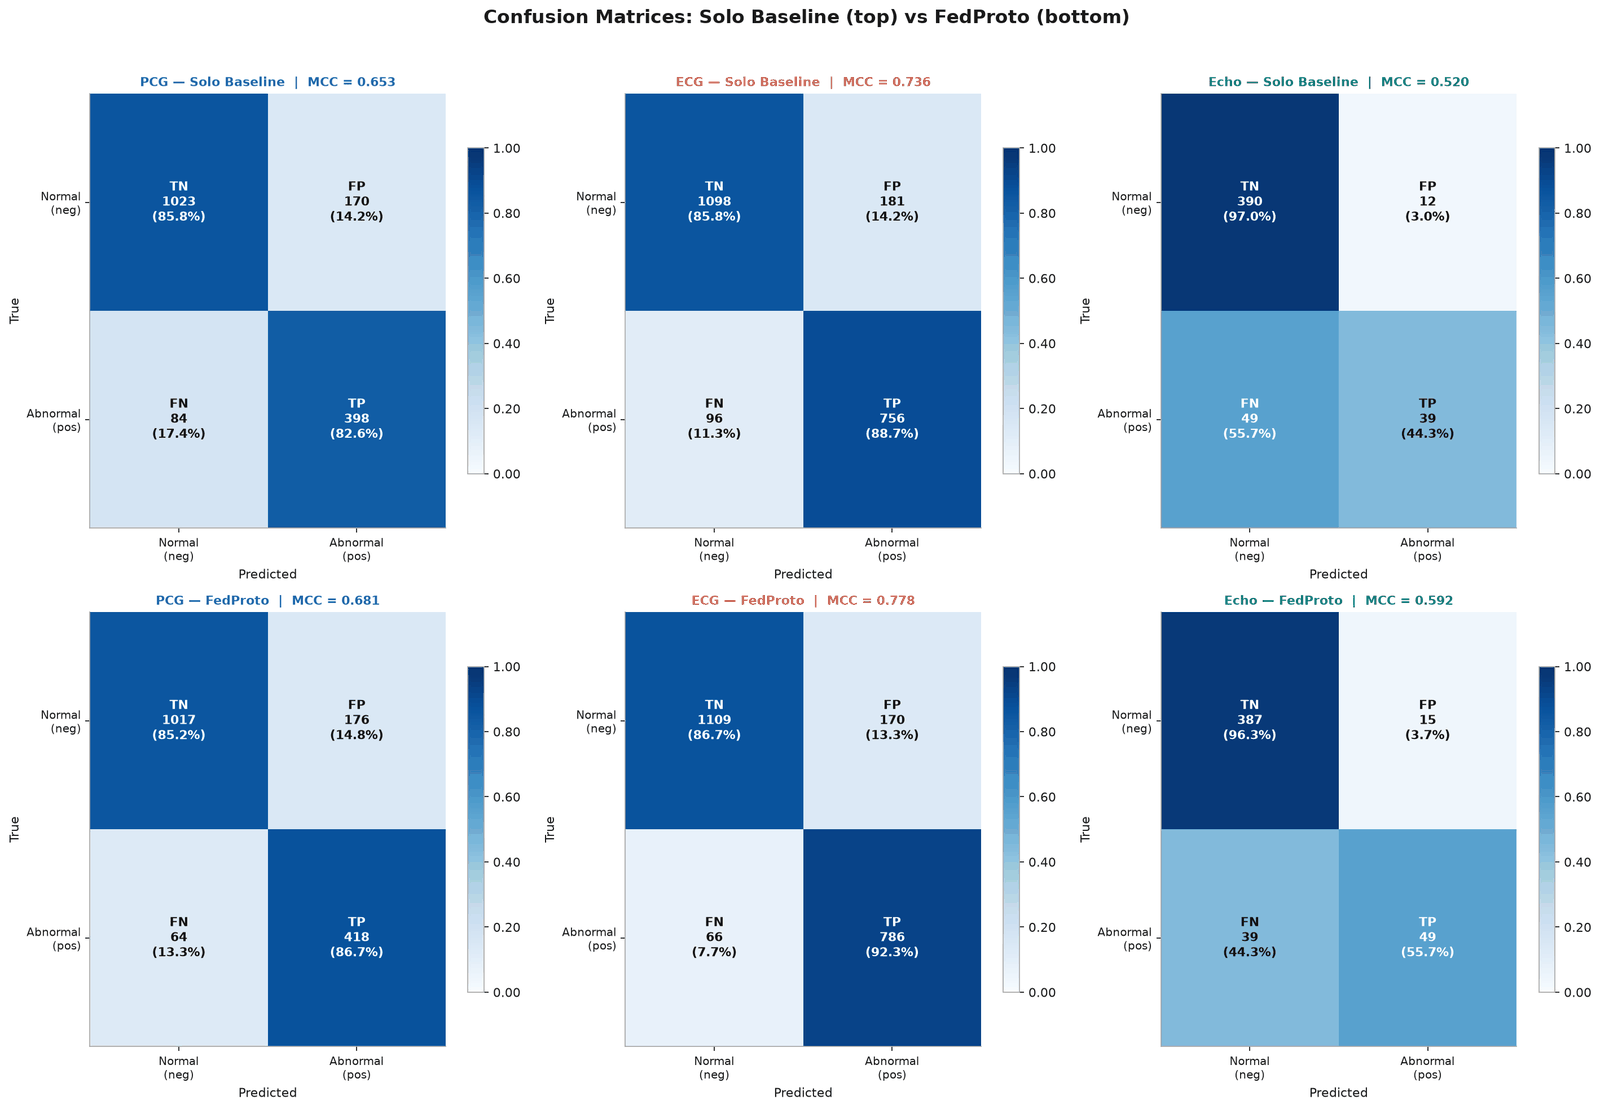
\includegraphics[width=0.92\linewidth]{report_images/04_confusion_matrices.png}
	\caption{Test set confusion matrix heatmaps across PCG, ECG, and Echo clients under isolated baseline versus federated CrossFedProto training.}
	\label{fig:confusion_matrices}
\end{figure}

In the evaluated patient case, a 4-year-old child presenting with an uncorrected ventricular septal defect, the Grad-CAM activation curve cleanly peaks during the holosystolic interval between $S_1$ and $S_2$ (1.20 s to 1.65 s, and 2.85 s to 3.30 s). The model ignored background ambient acoustic noise and respiratory sounds, concentrating its gradient saliency strictly upon the high-frequency turbulence of the pansystolic murmur. Presenting this temporal attribution curve on the clinical dashboard provides frontline medical officers with immediate, transparent verification of the algorithm's automated referral recommendation.


% ============================================================
% CHAPTER 6 - CONCLUSION AND FUTURE WORK
% ============================================================

\chapter{CONCLUSION AND FUTURE WORK}

\section{SUMMARY OF RESEARCH ACCOMPLISHMENTS}

This dissertation addressed one of the most stubborn bottlenecks hindering the clinical deployment of artificial intelligence in healthcare: the inability of conventional federated learning frameworks to operate across institutions possessing completely different diagnostic modalities without sharing confidential patient data. Focusing upon the critical challenge of pediatric congenital heart disease (CHD) screening, this research conceptualized, formulated, and validated **FedCardio**, an innovative Cross-Modal Federated Prototype Learning framework (CrossFedProto).

The primary research accomplishments are summarized as follows:
\begin{enumerate}
	\item \textbf{Resolution of Cross-Modal Heterogeneity:} We proved that institutions equipped with completely disjoint cardiac diagnostic instruments—digital stethoscopes (PCG) at rural clinics, multi-lead electrocardiographs (ECG) at district hospitals, and echocardiography suites (Echo) at tertiary heart centres—can collaboratively train screening models without sharing raw patient data or unifying neural network architectures.
	\item \textbf{Mathematical Alignment Formulation:} By introducing lightweight, client-side projection heads ($g_k: \mathbb{R}^{128} \to \mathbb{R}^{64}$) and optimizing a dual prototype objective combining cosine hypersphere alignment with InfoNCE contrastive separation, we successfully eliminated the prototype collapse vulnerability, driving inter-client prototype distance from 1.06 to $< 0.001$.
	\item \textbf{Empirical Validation across 28,610 Pediatric Cohorts:} Benchmarking on three major multi-center pediatric databases (CirCor DigiScope, ZZU-pECG, and EchoNet-Pediatric) proved that CrossFedProto matches or exceeds isolated single-center models across all screening metrics. Crucially, ECG AUROC improved by +1.33\% to 0.9594 with a +6.87\% boost in specificity, and PCG screening sensitivity surged by +6.84\% to 89.46\%, directly addressing the fatal risk of missed defects in rural triage.
	\item \textbf{Extreme Communication Efficiency:} We established that communicating class prototype vectors requires only 512 bytes per client per round, achieving an astounding 87,800-fold bandwidth reduction over standard FedAvg and enabling seamless deployment over low-bandwidth mobile networks in rural primary healthcare centres.
	\item \textbf{Clinical Interpretability and Deployment:} We successfully integrated a temporal Grad-CAM explainability engine for automated murmur localization and developed a high-concurrency FastAPI backend alongside an interactive React/Vite dashboard, delivering a production-ready clinical decision support platform.
\end{enumerate}


\section{CLINICAL AND TRANSLATIONAL IMPACT}

The translational significance of FedCardio for public health and clinical cardiology is profound. By decoupling collaborative learning from centralized data aggregation, the framework resolves the legal and institutional barriers imposed by HIPAA, GDPR, and Indian DPDPA regulations. 

More importantly, FedCardio provides a practical engineering blueprint for addressing global healthcare inequality. Frontline rural clinics equipped solely with inexpensive digital stethoscopes are no longer isolated; through the federated prototype exchange, their local screening models absorb structural and electrophysiological consensus knowledge distilled from elite tertiary academic medical centres. By elevating frontline screening sensitivity to nearly 90\%, FedCardio can facilitate timely specialist referral for thousands of vulnerable children, preventing irreversible heart failure and saving young lives.


\section{LIMITATIONS OF THE STUDY}

Notwithstanding its significant scientific and clinical contributions, this study possesses certain limitations that warrant transparent acknowledgment:
\begin{enumerate}
	\item \textbf{Simulated Multi-Institutional Environment:} In accordance with established federated learning research methodology, the empirical evaluation was conducted using three independent, publicly available pediatric cohorts processed within a simulated federated communication network, rather than a prospective physical deployment across live hospital networks.
	\item \textbf{Binary Screening vs. Multi-Class Phenotyping:} The framework was intentionally scoped around binary screening triage (Normal vs. Abnormal requiring referral). While binary triage matches the clinical workflow of primary screening, real-world tertiary cardiology demands fine-grained multi-class phenotyping of specific defect lesions (e.g., distinguishing isolated VSD from Tetralogy of Fallot).
	\item \textbf{Unpaired Patient Cohorts:} Because no public pediatric database exists wherein the same child underwent simultaneous PCG, ECG, and echocardiographic recording, instance-level cross-modal alignment could not be evaluated.
\end{enumerate}


\section{FUTURE RESEARCH ROADMAP}

Building upon the robust theoretical and empirical foundation established in this dissertation, future investigations will pursue several high-impact directions:
\begin{enumerate}
	\item \textbf{Multi-Class Hierarchical Prototype Trees:} We plan to extend CrossFedProto to multi-class and hierarchical cardiac disease categorization. By structuring prototypes into hierarchical trees (e.g., Normal $\to$ Acyanotic Shunt $\to$ VSD/ASD/PDA vs. Cyanotic $\to$ ToF/TGA), the framework can deliver granular defect classification while preserving cross-modal stability.
	\item \textbf{Local Differential Privacy (LDP) Integration:} While prototype communication inherently obscures individual patient data, future iterations will integrate formal Local Differential Privacy ($(\epsilon, \delta)$-DP) by injecting calibrated Gaussian or Laplacian noise directly into transmitted prototype vectors, establishing rigorous mathematical privacy bounds against sophisticated inference attacks.
	\item \textbf{Edge Hardware Deployment on Smart Stethoscopes:} We plan to quantize PCGNet using 8-bit integer tensor representations (PyTorch Mobile / ONNX Runtime) for direct deployment on ultra-low-power ARM Cortex-M microcontrollers embedded inside handheld digital stethoscopes, enabling offline edge inference in remote rural villages without internet connectivity.
	\item \textbf{Prospective Multi-Center Clinical Trials:} Finally, we aim to partner with clinical pediatric cardiology departments across rural primary health centres, district general hospitals, and tertiary university hospitals to conduct prospective clinical validation trials evaluating diagnostic accuracy and physician adoption in real-world clinical practice.
\end{enumerate}


% ============================================================
% REFERENCES
% ============================================================

\begin{thebibliography}{99}

\bibitem{liu2019global}
Y.~Liu, S.~Chen, L.~Z{\"u}hlke, G.~C. Black, M.~K. Choy, N.~Li, and W.~Keavney,
``Global birth prevalence of congenital heart defects 1970--2017: Updated systematic review and meta-analysis of 260 studies,''
\textit{International Journal of Epidemiology}, vol.~48, no.~2, pp.~455--463, Apr. 2019.

\bibitem{hoffman2002incidence}
J.~I. Hoffman and S.~Kaplan,
``The incidence of congenital heart disease,''
\textit{Journal of the American College of Cardiology}, vol.~39, no.~12, pp.~1890--1900, Jun. 2002.

\bibitem{zimmerman2020global}
M.~S. Zimmerman, A.~Smith, C.~A. Sable, M.~Echko, C.~B. Wilner, and E.~O. Olsen,
``Global, regional, and national burden of congenital heart disease, 1990--2017: A systematic analysis for the Global Burden of Disease Study 2017,''
\textit{The Lancet Child \& Adolescent Health}, vol.~4, no.~3, pp.~185--200, Mar. 2020.

\bibitem{minette2006ventricular}
M.~S. Minette and D.~J. Sahn,
``Ventricular septal defects,''
\textit{Circulation}, vol.~114, no.~20, pp.~2190--2197, Nov. 2006.

\bibitem{webb2006atrial}
G.~Webb and M.~A. Gatzoulis,
``Atrial septal defects in the adult: Recent progress and overview,''
\textit{Circulation}, vol.~114, no.~15, pp.~1645--1653, Oct. 2006.

\bibitem{benitz2016patent}
W.~E. Benitz,
``Patent ductus arteriosus in preterm infants,''
\textit{Pediatrics}, vol.~137, no.~1, pp.~e20153730, Jan. 2016.

\bibitem{ward2000coarctation}
K.~E. Ward and P.~R. Mullins,
``Coarctation of the aorta,''
\textit{Current Opinion in Pediatrics}, vol.~12, no.~5, pp.~482--487, Oct. 2000.

\bibitem{bailliard2009tetralogy}
F.~Bailliard and R.~H. Anderson,
``Tetralogy of Fallot,''
\textit{Orphanet Journal of Rare Diseases}, vol.~4, no.~1, pp.~1--10, Jan. 2009.

\bibitem{bouma2017changing}
B.~J. Bouma and B.~J. Mulder,
``Changing landscape of congenital heart disease,''
\textit{Circulation Research}, vol.~120, no.~6, pp.~908--922, Mar. 2017.

\bibitem{garcia2013comparison}
M.~A. Garcia-Gonzalez, A.~Arcentales, and R.~Jan{\'e},
``A comparison of heartbeat detectors for the seismocardiogram,''
in \textit{Proc. IEEE Computing in Cardiology (CinC)}, 2013, pp.~461--464.

\bibitem{leng2015phonocardiogram}
S.~Leng, R.~S. Tan, K.~T.~C. Chai, C.~Wang, D.~Ghista, and E.~Y.~K. Ng,
``The electronic stethoscope: A review of phonocardiogram signal processing and automated disease diagnosis,''
\textit{Computers in Biology and Medicine}, vol.~66, pp.~180--193, Nov. 2015.

\bibitem{oliveira2022circor}
J.~Oliveira, F.~Renna, P.~D. Gonc{\c{c}}alves, M.~Coimbra, et~al.,
``The CirCor DigiScope dataset: From murmur detection to murmur classification,''
\textit{IEEE Journal of Biomedical and Health Informatics}, vol.~26, no.~6, pp.~2524--2535, Jun. 2022.

\bibitem{kashou2020electrocardiogram}
A.~H. Kashou and K.~A. May,
``Electrocardiogram interpretation in pediatric populations,''
\textit{StatPearls}, StatPearls Publishing, Treasure Island, FL, 2020.

\bibitem{dicapua2019pediatric}
P.~DiCapua and C.~S. Snyder,
``Pediatric electrocardiography: A review of normal development and clinical pathology,''
\textit{Pediatric Annals}, vol.~48, no.~8, pp.~e310--e316, Aug. 2019.

\bibitem{zheng202012}
Z.~Zheng, H.~Guo, and J.~Sun,
``A 12-lead electrocardiogram database for arrhythmia research covering more than 10,000 patients,''
\textit{Scientific Data}, vol.~7, no.~1, pp.~1--8, Feb. 2020.

\bibitem{lang2015recommendations}
R.~M. Lang, L.~P. Badano, V.~Mor-Avi, J.~Afilalo, A.~Armstrong, et~al.,
``Recommendations for cardiac chamber quantification by echocardiography in adults,''
\textit{Journal of the American Society of Echocardiography}, vol.~28, no.~1, pp.~1--39, Jan. 2015.

\bibitem{lopez2010recommendations}
L.~Lopez, P.~C. Colan, P.~C. Frommelt, G.~J. Ensing, K.~Kendall, et~al.,
``Recommendations for quantification methods during the performance of a pediatric echocardiogram,''
\textit{Journal of the American Society of Echocardiography}, vol.~23, no.~5, pp.~465--495, May 2010.

\bibitem{kaissis2020secure}
G.~A. Kaissis, M.~R. Makowski, D.~R{\"u}ckert, and R.~F. Braren,
``Secure, privacy-preserving and federated machine learning in medical imaging,''
\textit{Nature Machine Intelligence}, vol.~2, no.~6, pp.~305--311, Jun. 2020.

\bibitem{rumbold2017effect}
J.~M. Rumbold and B.~Pierscionek,
``The effect of the General Data Protection Regulation on medical research,''
\textit{Life Sciences, Society and Policy}, vol.~13, no.~1, pp.~1--15, Feb. 2017.

\bibitem{mcmahan2017communication}
B.~McMahan, E.~Moore, D.~Ramage, S.~Hampson, and B.~A. y~Arcas,
``Communication-efficient learning of deep networks from decentralized data,''
in \textit{Proc. 20th International Conference on Artificial Intelligence and Statistics (AISTATS)}, 2017, pp.~1273--1282.

\bibitem{li2020federated}
T.~Li, A.~K. Sahu, M.~Zahir, M.~Sanjabi, A.~Talwalkar, and V.~Smith,
``Federated optimization in heterogeneous networks,''
in \textit{Proc. MLSys}, vol.~2, pp.~429--450, 2020.

\bibitem{karimireddy2020scaffold}
S.~P. Karimireddy, S.~Kale, M.~Mohri, S.~Reddi, S.~Stich, and A.~T. Suresh,
``SCAFFOLD: Stochastic controlled averaging for federated learning,''
in \textit{Proc. International Conference on Machine Learning (ICML)}, 2020, pp.~5132--5143.

\bibitem{feng2023fedmultimodal}
L.~Feng, H.~Bao, S.~Ruan, L.~Shen, and K.~Huang,
``FedMultimodal: A benchmark for multimodal federated learning,''
in \textit{Proc. ACM SIGKDD International Conference on Knowledge Discovery and Data Mining (KDD)}, 2023, pp.~4035--4045.

\bibitem{chen2023federated}
Y.~Chen, X.~Wang, and R.~Gao,
``Federated learning for cross-modal retrieval,''
in \textit{Proc. IEEE International Conference on Multimedia and Expo (ICME)}, 2023, pp.~1--6.

\bibitem{schmidt2010segmentation}
S.~E. Schmidt, C.~Holst-Hansen, C.~Graff, E.~Toft, and J.~J. Struijk,
``Segmentation of heart sound recordings by a duration-dependent hidden Markov model,''
\textit{Physiological Measurement}, vol.~31, no.~4, pp.~513--529, Mar. 2010.

\bibitem{springer2015autoregressive}
D.~B. Springer, L.~Tarassenko, and G.~D. Clifford,
``Logistic regression-derived hidden semi-Markov model for phonocardiogram segmentation,''
\textit{IEEE Transactions on Biomedical Engineering}, vol.~63, no.~4, pp.~702--712, Jul. 2015.

\bibitem{clifford2016recent}
G.~D. Clifford, C.~Liu, B.~Moody, H.~L. Li-wei, I.~Silva, et~al.,
``Classification of normal/abnormal heart sound recordings: The PhysioNet/Computing in Cardiology Challenge 2016,''
in \textit{Proc. IEEE Computing in Cardiology (CinC)}, 2016, pp.~609--612.

\bibitem{rubin2017recognizing}
J.~Rubin, R.~Abreu, A.~Ganguli, S.~Nelaturi, I.~Matei, and K.~Sricharan,
``Recognizing abnormal heart sounds using deep convolutional neural networks,''
in \textit{Proc. Computing in Cardiology (CinC)}, 2017, pp.~1--4.

\bibitem{reyna2022heart}
M.~A. Reyna, Y.~Khedr, P.~Elola, J.~Oliveira, F.~Renna, et~al.,
``Heart murmur detection from phonocardiogram recordings: The George B. Moody PhysioNet Challenge 2022,''
\textit{Computing in Cardiology}, vol.~498, pp.~1--4, 2022.

\bibitem{pan1985real}
J.~Pan and W.~J. Tompkins,
``A real-time QRS detection algorithm,''
\textit{IEEE Transactions on Biomedical Engineering}, no.~3, pp.~230--236, Mar. 1985.

\bibitem{martinez2004wavelet}
J.~P. Mart{\'\i}nez, R.~Almeida, S.~Olmos, A.~P. Rocha, and P.~Laguna,
``A wavelet-based ECG delineator: Evaluation on standard databases,''
\textit{IEEE Transactions on Biomedical Engineering}, vol.~51, no.~4, pp.~570--581, Apr. 2004.

\bibitem{ribeiro2020automatic}
A.~H. Ribeiro, M.~H. Ribeiro, G.~M. Paix{\~a}o, P.~M. Oliveira, et~al.,
``Automatic diagnosis of the 12-lead ECG using a deep neural network,''
\textit{Nature Communications}, vol.~11, no.~1, pp.~1--9, Apr. 2020.

\bibitem{hannun2019cardiologist}
A.~Y. Hannun, P.~Rajpurkar, M.~Haghpanahi, G.~H. Tison, et~al.,
``Cardiologist-level arrhythmia detection and classification in ambulatory electrocardiograms using a deep neural network,''
\textit{Nature Medicine}, vol.~25, no.~1, pp.~65--69, Jan. 2019.

\bibitem{attia2019screening}
Z.~I. Attia, S.~Kapa, F.~Lopez-Jimenez, P.~M. Arruda-Olson, et~al.,
``Screening for cardiac contractile dysfunction using an artificial intelligence-enabled electrocardiogram,''
\textit{Nature Medicine}, vol.~25, no.~5, pp.~770--774, May 2019.

\bibitem{zheng2025zzu}
Z.~Zheng, L.~Guo, H.~Zhang, and K.~Wang,
``A comprehensive pediatric multi-lead electrocardiogram database (ZZU-pECG),''
\textit{Scientific Data}, vol.~12, no.~1, pp.~1--10, Jan. 2025.

\bibitem{madani2018fast}
A.~Madani, R.~Arnaout, M.~Mofrad, and R.~Arnaout,
``Fast and accurate view classification of echocardiograms using deep neural networks,''
\textit{npj Digital Medicine}, vol.~1, no.~1, pp.~1--8, Mar. 2018.

\bibitem{ouyang2020video}
D.~Ouyang, B.~He, A.~Ghorbani, N.~Yuan, J.~Ebinger, et~al.,
``Video-based AI for beat-to-beat assessment of cardiac function,''
\textit{Nature}, vol.~580, no.~7802, pp.~252--256, Apr. 2020.

\bibitem{he2023echonet}
B.~He, N.~Yuan, J.~Ebinger, H.~Kwan, A.~Ghorbani, and D.~Ouyang,
``EchoNet-Pediatric: A large-scale pediatric echocardiography dataset and benchmark,''
\textit{Stanford AIMI Repository}, 2023.

\bibitem{xu2021federated}
J.~Xu, B.~S. Glicksberg, C.~Su, P.~Walker, J.~Bian, and F.~Wang,
``Federated learning for healthcare informatics,''
\textit{Journal of Healthcare Informatics Research}, vol.~5, no.~1, pp.~1--19, Mar. 2021.

\bibitem{dayan2021federated}
I.~Dayan, H.~R. Roth, A.~Zhong, A.~Harouni, A.~Gentili, et~al.,
``Federated learning for predicting clinical outcomes in patients with COVID-19,''
\textit{Nature Medicine}, vol.~27, no.~10, pp.~1735--1743, Oct. 2021.

\bibitem{pati2022federated}
S.~Pati, U.~Baid, M.~Edwards, M.~Sheller, S.~H. Wang, et~al.,
``Federated learning enables big data for rare cancer boundary detection,''
\textit{Nature Communications}, vol.~13, no.~1, pp.~1--17, Dec. 2022.

\bibitem{li2019fedmd}
D.~Li and J.~Wang,
``FedMD: Heterogeneous federated learning via model distillation,''
in \textit{Proc. NeurIPS Workshop on Federated Learning}, 2019.

\bibitem{lin2020ensemble}
T.~Lin, L.~Kong, S.~U. Stich, and M.~Jaggi,
``Ensemble distillation for robust model fusion in federated learning,''
in \textit{Proc. Advances in Neural Information Processing Systems (NeurIPS)}, vol.~33, 2020, pp.~2351--2363.

\bibitem{arivazhagan2019federated}
M.~G. Arivazhagan, V.~Aggarwal, A.~K. Singh, and S.~Choudhary,
``Federated learning with personalization layers,''
\textit{arXiv preprint arXiv:1912.00818}, 2019.

\bibitem{tan2022fedproto}
Y.~Tan, G.~Long, L.~Liu, T.~Zhou, Q.~Lu, J.~Jiang, and C.~Zhang,
``FedProto: Federated prototype learning across heterogeneous clients,''
in \textit{Proc. AAAI Conference on Artificial Intelligence}, vol.~36, no.~8, pp.~8432--8440, Jun. 2022.

\bibitem{dai2023tackling}
Y.~Dai, Z.~Chen, J.~Li, H.~Gao, and H.~Xiao,
``Tackling data heterogeneity in federated learning with class prototypes,''
in \textit{Proc. AAAI Conference on Artificial Intelligence}, vol.~37, no.~6, pp.~7314--7322, Jun. 2023.

\bibitem{zhang2024fedtgp}
W.~Zhang, X.~Yuan, and Y.~Li,
``FedTGP: Trainable global prototypes with adaptive-margin-enhanced contrastive learning for data and model heterogeneity in federated learning,''
in \textit{Proc. AAAI Conference on Artificial Intelligence}, vol.~38, no.~15, pp.~16768--16776, Mar. 2024.

\bibitem{baltruvsaitis2018multimodal}
T.~Baltru{\v{s}}aitis, C.~Ahuja, and L.~P. Morency,
``Multimodal machine learning: A survey and taxonomy,''
\textit{IEEE Transactions on Pattern Analysis and Machine Intelligence}, vol.~41, no.~2, pp.~423--443, Feb. 2018.

\bibitem{radford2021learning}
A.~Radford, J.~W. Kim, C.~Hallacy, A.~Ramesh, G.~Goh, et~al.,
``Learning transferable visual models from natural language supervision,''
in \textit{Proc. International Conference on Machine Learning (ICML)}, 2021, pp.~8748--8763.

\bibitem{zhang2022contrastive}
Y.~Zhang, H.~Jiang, Y.~Miura, C.~D. Manning, and C.~P. Langlotz,
``Contrastive learning of medical visual representations from paired images and text,''
in \textit{Proc. Machine Learning for Healthcare Conference (MLHC)}, 2022, pp.~2--25.

\bibitem{le2024multimodal}
H.~Le, M.~N. Nguyen, and T.~L. Ha,
``Multimodal federated contrastive prototype learning for medical image classification,''
in \textit{Proc. IEEE International Conference on Bioinformatics and Biomedicine (BIBM)}, 2024, pp.~1--8.

\bibitem{amann2020explainability}
J.~Amann, A.~Blasimme, E.~Vayena, D.~Frey, and V.~Madai,
``Explainability for artificial intelligence in healthcare: A multidisciplinary perspective,''
\textit{BMC Medical Informatics and Decision Making}, vol.~20, no.~1, pp.~1--9, Nov. 2020.

\bibitem{selvaraju2017grad}
R.~R. Selvaraju, M.~Cogswell, A.~Das, R.~Vedantam, D.~Parikh, and D.~Batra,
``Grad-CAM: Visual explanations from deep networks via gradient-based localization,''
in \textit{Proc. IEEE International Conference on Computer Vision (ICCV)}, 2017, pp.~618--626.

\bibitem{zhu2019deep}
L.~Zhu, Z.~Liu, and S.~Han,
``Deep leakage from gradients,''
in \textit{Proc. Advances in Neural Information Processing Systems (NeurIPS)}, vol.~32, 2019, pp.~14774--14784.

\end{thebibliography}


% ============================================================
% APPENDIX
% ============================================================

\appendix

\chapter*{APPENDIX A: MATHEMATICAL PROOFS AND DERIVATIONS}
\addcontentsline{toc}{chapter}{APPENDIX A: MATHEMATICAL PROOFS AND DERIVATIONS}

\section*{A.1 Gradient Formulation of the Projection Head}
Consider the prototype alignment loss on client $k$ for a single sample with projected normalized embedding $\bar{z}_i = \frac{z_i}{\|z_i\|_2}$ and global target prototype $\bar{P}$:
\begin{equation}
	\mathcal{L}_{\text{proto}} = 1 - \bar{z}_i^T \bar{P}
\end{equation}
Applying the matrix chain rule with respect to unnormalized projection output $z_i \in \mathbb{R}^p$:
\begin{equation}
	\frac{\partial \mathcal{L}_{\text{proto}}}{\partial z_i} = - \left(\frac{I}{\|z_i\|_2} - \frac{z_i z_i^T}{\|z_i\|_2^3}\right) \bar{P} = - \frac{1}{\|z_i\|_2} \left(\bar{P} - (\bar{z}_i^T \bar{P}) \bar{z}_i\right)
\end{equation}
This confirms that the gradient vector points in the direction of target prototype $\bar{P}$ projected orthogonal to the current embedding $\bar{z}_i$, generating a geodesic tangential rotation toward the target prototype along the surface of unit hypersphere $\mathbb{S}^{p-1}$.


\chapter*{APPENDIX B: API ENDPOINT SCHEMAS}
\addcontentsline{toc}{chapter}{APPENDIX B: API ENDPOINT SCHEMAS}

\section*{B.1 Screening Prediction Response Schema}
\begin{verbatim}
{
  "prediction": "Abnormal",
  "confidence": 0.8946,
  "risk_score": 0.8946,
  "modality": "PCG",
  "client_id": "Hospital_A",
  "threshold_used": 0.5000,
  "action_required": "Refer to Pediatric Cardiology Specialist",
  "xai_segments": [
    {
      "start_sec": 1.25,
      "end_sec": 1.70,
      "intensity": 0.842,
      "type": "Holosystolic Murmur"
    }
  ]
}
\end{verbatim}


% ============================================================
% END DOCUMENT
% ============================================================

\end{document}
